\subsection{Hopf spaces}

DEFINITION 2. --- A Hopf space is a pointed topological space (X, e) equipped with a continuous composition law m: X × X → X such that

\begin{enumerate}
\def\labelenumi{(\roman{enumi})}
\item
  \(m(e, e) = e\) ;
\item
  there exist pointed homotopies at \(e\) relating the maps \(x \mapsto m(x, e)\) and \(x \mapsto m(e, x)\) to the map \(\mathrm{Id}_{\mathrm{X}}\) .
\end{enumerate}

One sometimes expresses properties (i) and (ii) by saying that e is a neutral element up to homotopy for the composition law m.

Note that there may exist several identity elements up to homotopy for a continuous composition law m on a topological space X. For example, for \(X = \mathbf{R}\) and \(m(x, y) = (x + y)/2\) , every \(x \in \mathbf{R}\) is a neutral element up to homotopy.

Examples. --- 1) Let G be a topological group and m its composition law. The identity element e of G is an identity element up to homotopy, and (G, e) is a Hopf space.

\begin{enumerate}
\def\labelenumi{\arabic{enumi})}
\setcounter{enumi}{1}
\tightlist
\item
  Let X be a topological space and let x be a point of X. Equipped with the concatenation of loops at x, the pointed space \((\Omega_{x}(\mathrm{X}), e_{x})\) is a Hopf space. Indeed, one first has \(e_{x} * e_{x} = e_{x}\). On the other hand, let \(\psi: I \to I\) be the function defined by \(\psi(t) = 2t\) for \(0 \leqslant t \leqslant \frac{1}{2}\) and \(\psi(t) = 1\) for \(\frac{1}{2} \leqslant t \leqslant 1\) (cf. III, p.~291), and let \(\sigma: I \times I \to I\) be a strict homotopy joining \(\psi\) to \(\mathrm{Id}_{\mathrm{I}}\) (III, p.~289, example). Then, for every loop \(c \in \Omega_{x}(\mathrm{X})\) , the map \(c \circ \sigma: I \times I \to X\) is a strict homotopy joining \(c * e_{x}\) to c in \(\Omega_{x}(\mathrm{X})\) .
\end{enumerate}

Let \(\tau\) be the map \(\Omega_x(\mathrm{X}) \times \mathbf{I} \to \Omega_x(\mathrm{X})\) defined by \(\tau(c, s)(t) = c \circ \sigma(s, t)\) . Let us prove that \(\tau\) is continuous. By Proposition 1 of III, p.~257, it suffices to show that the map \((c, s, t) \mapsto c(\sigma(s, t))\) from \(\Omega_x(\mathrm{X}) \times \mathbf{I} \times \mathbf{I}\) into X is continuous, that is, since \(\mathbf{I} \times \mathbf{I}\) is compact, that the map \(c \mapsto c \circ \sigma\) from \(\mathcal{C}_c(\mathbf{I};\mathrm{X})\) into \(\mathcal{C}_c(\mathbf{I} \times \mathbf{I};\mathrm{X})\) is continuous. This last assertion then follows from the lemma, I, p.~132, b). Consequently, the map \(\tau\) is a homotopy connecting the map \(c \mapsto c * e_x\) to the identity map of \(\Omega_x(\mathrm{X})\) . We have \(\tau(e_x, s)(t) = x\) for all \(s, t \in I\) , therefore \(\tau\) is a pointed homotopy at \(e_x\). One argues similarly for the map \(c \mapsto e_x * c\) .

PROPOSITION 3. — Let (X, e) be a Hopf space and m: X × X → X its composition law. For all loops c, c′ in X at e, one has:

\[
c ^ {\prime} * c \sim c * c ^ {\prime} \sim m \circ (c, c ^ {\prime}),
\]

where ∼ denotes the strict homotopy relation. The composition law of the group \(\pi_{1}(\mathrm{X},e)\) is the composite of the canonical isomorphism \(\pi_{1}(\mathrm{X},e)\times\pi_{1}(\mathrm{X},e)\to\pi_{1}(\mathrm{X}\times\mathrm{X},(e,e))\) (III, p.~297, corollary) and the homomorphism \(\pi_{1}(m,(e,e))\) from \(\pi_{1}(\mathrm{X}\times\mathrm{X},(e,e))\) into \(\pi_{1}(\mathrm{X},e)\) . The group \(\pi_{1}(\mathrm{X},e)\) is commutative.

Let \(\mu\colon\pi_{1}(\mathrm{X},e)\times\pi_{1}(\mathrm{X},e)\to\pi_{1}(\mathrm{X},e)\) be the group homomorphism given by the composite of the canonical isomorphism of \(\pi_{1}(\mathrm{X},e)\times\pi_{1}(\mathrm{X},e)\) onto \(\pi_{1}(\mathrm{X}\times\mathrm{X},(e,e))\) and the homomorphism \(\pi_{1}(m,(e,e))\) . It remains to prove that one has

\[
\mu (\gamma , \gamma^ {\prime}) = \gamma \gamma^ {\prime} = \gamma^ {\prime} \gamma\tag{1}
\]

for all \(\gamma, \gamma' \in \pi_1(X, e)\) . In view of remark 2 of III, p.~297, we have:

\[
\mu (\gamma , \gamma^ {\prime}) = \mu (\gamma , \varepsilon_ {e}) \mu (\varepsilon_ {e}, \gamma^ {\prime}) = \mu (\varepsilon_ {e}, \gamma^ {\prime}) \mu (\gamma , \varepsilon_ {e}).\tag{2}
\]

Let \(c \in \Omega_e(\mathrm{X})\) be a loop of class \(\gamma\) , and denote by \(m_1 \colon \mathrm{X} \to \mathrm{X}\) the map defined by \(m_1(x) = m(x, e)\) ; then, \(\mu(\gamma, \varepsilon_e)\) is the class of \(m_1 \circ c\) . By definition of a Hopf space, the pointed maps at \(e\) , \(m_1\) and \(\mathrm{Id_X}\) have the same pointed homotopy class at \(e\) . Consequently, the loops at \(e\) , \(m_1 \circ c\) and \(c\) are strictly homotopic (III, p.~296, cor. 1 of prop. 3) and one has \(\mu(\gamma, \varepsilon_e) = \gamma\) . One proves in an analogous way that one has \(\mu(\varepsilon_e, \gamma') = \gamma'\) . Relation (1) then follows from relation (2).

Note. --- Let \((X,e)\) be a Hopf space. By prop. 3, the composition map of path classes, \(\pi_{1}(X,e)\times\pi_{1}(X,e)\to\pi_{1}(X,e)\) is continuous if \(\pi_{1}(X,e)\) is equipped with the quotient topology of the compact-convergence topology on \(\Lambda_{e}(X)\) . This is indeed the composite of the continuous isomorphism \(\pi_{1}(X,e)\times\pi_{1}(X,e)\to\pi_{1}(X\times X,(e,e))\) (III, p.~298, remark 3) and the continuous map \(m_{*}:\pi_{1}(X\times X,(e,e))\to\pi_{1}(X,e)\) (III, p.~294, remark 1).

\subsection{Poincaré group of topological groups}

If G is a topological group, for every \(g \in G\) , the left translation \(x \mapsto gx\) is a homeomorphism of G onto itself (TG, III, p.~2) and it induces an isomorphism of \(\pi_{1}(G, e)\) onto \(\pi_{1}(G, g)\) .

Let G be a topological group, let e be its identity element, and denote by \(G_{0}\) the path-connected component of e in G. Denote by R the equivalence relation on G whose equivalence classes are the path-connected components of G, and let \(p: G \to \pi_{0}(G)\) be the canonical map. Since every translation, left or right, is a homeomorphism of G, the relation R is compatible on the left and on the right with the group law of G. By th. 2 of A, I, p.~35, the group \(G_{0}\) is a normal subgroup of G, the quotient group \(G/G_{0}\) is equal to \(\pi_{0}(G)\) endowed with the composition law induced by that of G, and the map p is a group homomorphism.

The group \(\pi_{1}(G,e)\) is called the Poincaré group of G and is denoted by \(\pi_{1}(G)\) . The canonical injection of \(G_{0}\) into G induces an isomorphism of \(\pi_{1}(G_{0})\) onto \(\pi_{1}(G)\) (III, p.~293, remark 2).

Let \(g\) be an element of G; the right translation \(\boldsymbol{\delta}_g \colon x \mapsto xg\) induces an isomorphism \((\boldsymbol{\delta}_g)_* \colon \pi_1(\mathrm{G}) \to \pi_1(\mathrm{G}, g)\) . Suppose that \(g\) belongs to \(\mathrm{G}_0\) and let \(b\) be a path connecting \(e\) to \(g\) . The map \(\sigma \colon \mathrm{G} \times \mathbf{I} \to \mathrm{G}\) defined by \(\sigma(x, t) = xb(t)\) is a homotopy connecting \(\mathrm{Id}_{\mathrm{G}}\) to \(\boldsymbol{\delta}_g\) . By prop. 3 of III, p.~295, one therefore has, for every \(\alpha \in \pi_1(\mathrm{G})\) , \((\boldsymbol{\delta}_g)_*(\alpha) = \beta^{-1}\alpha\beta\) , where \(\beta \in \varpi_{e,g}(\mathrm{G})\) is the class of the path \(b\) . If one denotes by \(\gamma_g\) the left translation, \(x \mapsto gx\) , one likewise has \((\gamma_g)_*(\alpha) = \beta^{-1}\alpha\beta\) .

For every \(g \in G\) , the map \(\operatorname{Int}(g)\) : \(G \to G\) induces an automorphism \(\pi_{1}(\operatorname{Int}(g))\) of \(\pi_{1}(G)\) . One thus defines an action of G on \(\pi_{1}(G)\) . For all \(g \in G\) , we have \(\pi_{1}(\operatorname{Int}(g)) = (\boldsymbol{\gamma}_{g^{-1}})_{*} \circ (\boldsymbol{\delta}_{g})_{*}\) , so that the subgroup \(G_{0}\) operates trivially; this yields an action of \(\pi_{0}(G)\) on \(\pi_{1}(G)\) . When G is a commutative group, this action is trivial, but this is not always the case (IV, p.~459, exerc. 1).

\subsection{Coverings of topological groups}

PROPOSITION 4. --- Let (X, e) be a Hopf space (IV, p.~373, definition 2) and let m: X × X → X be its composition law. Suppose the space X is connected and locally path-connected. Let X' be a connected covering of X; denote its projection by p and let e' be a point of the fiber \(X'_{e}\).

\begin{enumerate}
\def\labelenumi{\alph{enumi})}
\item
  The covering X' is Galois and its automorphism group is commutative.
\item
  There exists a unique continuous composition law \(m' \colon X' \times X' \to X'\) such that one has \(p \circ m' = m \circ (p, p)\) and \(m'(e', e') = e'\) . Endowed with this composition law, the pointed space \((X', e')\) is a Hopf space.
\item
  Endowed with the composition law induced by \(m'\), the fiber \(X'_e\) is a group with identity element \(e'\). The map from \(\pi_1(X, x)\) into \(X'_e\) given by \(\gamma \mapsto e' \cdot \gamma\) is a surjective group homomorphism with kernel \(p_*(\pi_1(X', e'))\) . The map \(g \mapsto g(e')\) is an isomorphism of the group \(\text{Aut}_X(X')\) onto the group \(X'_e\) .
\item
  The group \(\pi_{1}(X,e)\) is commutative (prop. 3). Since the covering \(X'\) of X is connected, it is then a Galois covering and the group \(\operatorname{Aut}_{\mathrm{X}}(\mathrm{X}')\) is isomorphic to the quotient group \(\pi_{1}(\mathrm{X},e)/p_{*}(\pi_{1}(\mathrm{X}',e'))\) (III, p.~312, corollary 4 of proposition 2); this group is commutative.
\item
  Denote by \(q\colon X^{\prime}\times X^{\prime}\to X\) the map \(m\circ (p,p)\) . The map \(m'\) required is a continuous lifting of \(q\) to \(X^{\prime}\) such that \(m'(e',e') = e'\) . The space \(X^{\prime}\times X^{\prime}\) is locally path-connected; it therefore suffices, in order to prove the existence of such a continuous lifting, to verify that \(q_{*}(\pi_{1}(X^{\prime}\times X^{\prime},(e^{\prime},e^{\prime})))\) is contained in \(p_{*}(\pi_{1}(X^{\prime},e^{\prime}))\) (III, p.~308, prop. 1). By prop. 3, the map \(\pi_1(m,(e,e))\) is identified with the composition law of the group \(\pi_1(X,e)\) when one identifies \(\pi_1(X\times X,(e,e))\) with \(\pi_1(X,e)\times \pi_1(X,e)\) . The group \(q_{*}(\pi_{1}(X^{\prime}\times X^{\prime},(e^{\prime},e^{\prime})))\) is therefore equal to the group \(p_{*}(\pi_{1}(X^{\prime},e^{\prime}))\) , whence the existence of \(m'\) . Since \(X^{\prime}\times X^{\prime}\) is connected, the uniqueness of \(m'\) follows from I, p.~34, corollary 1 of prop. 11.
\end{enumerate}

Let us prove that the map \(m'\) endows the pointed space \((\mathrm{X}', e')\) with a Hopf space structure. Let \(m_1 \colon X \to X\) be the map \(g \mapsto m(g, e)\) and let \(\sigma_1 \colon X \times I \to X\) be a pointed homotopy at x connecting \(m_1\) to \(Id_X\) . Set \(\tau = \sigma_1 \circ (p, \mathrm{Id_I}) \colon X' \times I \to X\) . The map \(m'_1 \colon X' \to X'\) defined by \(h \mapsto m'(h, e')\) lifts the map \(\tau(\cdot, 0)\) ; let \(\tau' \colon X' \times I \to X'\) be the lifting of \(\tau\) whose initial map is \(m'_1\) (III, p.~301, prop. 2). The map \(t \mapsto \tau'(e', t)\) is a lift to \(X'\) of the constant map \(t \mapsto e\) ; since \(\tau'(e', 0) = e'\) , we therefore have \(\tau'(e', t) = e'\) for all \(t \in I\) . The map \(\tau'(\cdot, 1)\) is then a lifting to \(X'\) of the map p which maps \(e'\) onto \(e'\) . Since \(X'\) is connected, \(Id_{X'}\) is the unique X-morphism from \(X'\) to itself that fixes the point \(e'\) ; one therefore has \(\tau'(\cdot,1)=\mathrm{Id}_{\mathrm{X}'}\) . This shows that \(\tau'\) is a pointed homotopy at \(e'\) which connects the map \(m_{1}'\) to the map \(Id_{X'}\) . Likewise, there exists a pointed homotopy at \(e'\) connecting the map \(m_{2}'\colon h\mapsto m'(e',h)\) to the map \(Id_{X'}\) . This proves that the pointed space ( \(X',e'\) ), equipped with the composition law \(m'\) , is a Hopf space.

\begin{enumerate}
\def\labelenumi{\alph{enumi})}
\setcounter{enumi}{2}
\tightlist
\item
  Since \(X'\) is a connected covering of X, the orbit map of \(e'\) induced by the action of \(\pi_{1}(\mathrm{X},e)\) on \(X'_{e}\) is surjective and induces a bijection from \(\pi_{1}(\mathrm{X},e)/p_{*}(\pi_{1}(\mathrm{X}',e'))\) onto \(X'_{e}\) (III, p.~305, Theorem 1).
\end{enumerate}

Let \(c\) and \(d\) be loops of X at \(e\) , and let \(\gamma\) and \(\delta \in \pi_1(\mathrm{X},e)\) be their classes. Let \(c'\) and \(d'\) be the paths with initial point \(e'\) on \(\mathrm{X}'\) which lift \(c\) and \(d\) . We have \(e' \cdot \gamma = c'(1)\) and \(e' \cdot \delta = d'(1)\) (III, p.~304). By Proposition 3 of IV, p.~374, the loop \(m \circ (c,d)\) is strictly homotopic to the loop \(c*d\) ; one therefore has \(e' \cdot (\gamma\delta) = e' \cdot (m \circ (c,d))\) . Now, the path \(m' \circ (c',d')\) is a lifting with origin \(e'\) of the path \(m \circ (c,d)\) ; one therefore has

\[
e ^ {\prime} \cdot (\gamma \delta) = m ^ {\prime} (c ^ {\prime} (1), d ^ {\prime} (1)) = m ^ {\prime} (e ^ {\prime} \cdot \gamma , e ^ {\prime} \cdot \delta).
\]

The map \(\gamma \mapsto e' \cdot \gamma\) is therefore a homomorphism from \(\pi_1(\mathrm{X}, e)\) into the set \(\mathrm{X}'_e\) endowed with the composition law induced by \(m'\) . Consequently, \(\mathrm{X}'_e\) is a group under the composition law induced by \(m'\) and the orbit map of \(e'\) is an isomorphism from the quotient group \(\pi_1(\mathrm{X}, e)/p_*(\pi_1(\mathrm{X}', e'))\) onto \(\mathrm{X}'_e\) .

The last part of assertion c) then follows from Corollary 3 of III, p.~311.

PROPOSITION 5. --- We retain the notation and hypotheses of Proposition 4.

\begin{enumerate}
\def\labelenumi{\alph{enumi})}
\item
  If m is an associative (respectively commutative) law of composition, then so is \(m'\) .
\item
  If e is a right identity element (resp. left identity element) for the operation m, then e' is a right identity element (resp. left identity element) for the operation m'.
\item
  If X is a topological group, m its composition law, and e its identity element, the composition law m' endows X' with a group structure compatible with the topology of X', with e' as its identity element. The map p: X' → X is a group homomorphism whose kernel is discrete and contained in the center of X'.
\item
  Suppose that the law m is associative. Then the maps from \(X' \times X' \times X'\) into X that send \((h_{1}, h_{2}, h_{3})\) to \(m(p(h_{1}),m(p(h_{2}),p(h_{3})))\) and \(m(m(p(h_{1}),p(h_{2})),p(h_{3}))\), respectively, are equal. The maps \((h_{1},h_{2},h_{3})\mapsto m'(h_{1},m'(h_{2},h_{3}))\) and \((h_{1},h_{2},h_{3})\mapsto m'(m'(h_{1},h_{2}),h_{3})\) from \(X'\times X'\times X'\) into \(X'\) are continuous lifts that coincide at the point \((e',e',e')\) . Since \(X'\times X'\times X'\) is connected, they are equal (I, p.~34, cor. 1 of prop. 11), which shows that the law \(m'\) is associative.
\end{enumerate}

Suppose now that the law \(m\) is commutative; the maps \((h_1, h_2) \mapsto m'(h_1, h_2)\) and \((h_1, h_2) \mapsto m'(h_2, h_1)\) are continuous lifts to \(X'\) of the map \((h_1, h_2) \mapsto m(p(h_1), p(h_2))\) which coincide at the point \((e', e')\) . Since \(X' \times X'\) is connected, they are equal (loc. cit.) and the law \(m'\) is commutative.

If \(e\) is a right (resp. left) identity element for the law \(m\) , the map \(h \mapsto m'(h, e')\) (resp. \(h \mapsto m'(e', h)\) ) from \(X'\) into \(X'\) is an X-morphism of coverings that coincides with \(\text{Id}_{X'}\) at the point \(e'\) , hence at every point of \(X'\) , since \(X'\) is connected (loc. cit.), whence \(b\) ).

Let us finally prove c). Suppose that X is a topological group. By the preceding, the law \(m'\) is associative and \(e'\) is a neutral element. Let us denote by \(i: X \to X\) the map \(g \mapsto g^{-1}\) . It is continuous (TG, III, p.~1) and the homomorphism \(\pi_{1}(i,e): \pi_{1}(X,e) \to \pi_{1}(X,e)\) is none other than the map \(\gamma \mapsto \gamma^{-1}\) (IV, p.~374, prop. 3). Consequently, the subgroup \((i \circ p)_{*}(\pi_{1}(X',e'))\) is equal to \(p_{*}(\pi_{1}(X',e'))\) . By prop. 1 of III, p.~308, there therefore exists a continuous map \(i': X' \to X'\) such that \(p \circ i' = i \circ p\) and \(i'(e') = e'\) . The maps \(h \mapsto m'(h,i'(h))\) and \(h \mapsto m'(i'(h),h)\) from \(X'\) into \(X'\) are liftings to \(X'\) of the constant map with image e from \(X'\) into X. They are therefore constant and their image is \(e' = m'(e',e')\) . Thus, every element h of \(X'\) is invertible, with inverse \(i'(h)\) , which shows that \(X'\) , equipped with the composition law \(m'\) , is a group. By construction of the law \(m'\) , the map p: \(X' \to X\) is a group homomorphism. Since the maps \(m'\) and \(i'\) are continuous, the group structure of \(X'\) is compatible with its topology (TG, III, p.~1). The fiber \(p^{-1}(e)\) is a discrete subgroup of \(X'\) which is contained in the center of \(X'\) (I, p.~100, cor. 3) and X is isomorphic to the quotient topological group \(X'/p^{-1}(e)\) .

COROLLARY. --- Let G be a connected and locally path-connected topological group. Let G' be a connected covering of G, let p be its projection, and let e' be an element of the fiber N of the identity element e of G. Endow G' with the unique continuous composition law m': G' × G' → G' such that \(p \circ m' = m \circ (p, p)\) and \(m'(e', e') = e'\) . If i: N → G' denotes the canonical injection, then (G', p, i) is a central extension of G by N (A, I, p.~63).

\subsection{Universal covering of a deloopable topological group}

Let G be a locally path-connected topological group. The translations of G are homeomorphisms (TG, III, p.~2). For the space G to be deloopable (IV, p.~340, def. 2), it is necessary and sufficient that G possess the following property:

There exists a neighborhood V of the identity element e of G such that the image of the homomorphism from \(\pi_{1}(V,e)\) into \(\pi_{1}(G,e)\) deduced from the canonical injection is reduced to the identity element.

PROPOSITION 6. --- Let G be a connected and deloopable topological group. There exists a topological group \(\widetilde{\mathbf{G}}\) with identity element \(\widetilde{e}\) , and a continuous homomorphism \(p\colon \widetilde{\mathbf{G}}\to \mathbf{G}\) satisfying the following assertions:

\begin{enumerate}
\def\labelenumi{\alph{enumi})}
\item
  The space \(\widetilde{G}\) is simply connected and simply path-connected. Equipped with the map p, the pointed space ( \(\widetilde{G},\widetilde{e}\) ) is a universal covering of the pointed space (G,e).
\item
  The kernel N of p is a discrete subgroup of \(\widetilde{G}\), contained in the center of \(\widetilde{G}\) . The homomorphism \(\mathrm{N}\to\mathrm{Aut}_{\mathrm{G}}(\widetilde{\mathrm{G}})\) which sends \(n\in N\) to the right translation in \(\widetilde{G}\) , is a group isomorphism. The homomorphism from \(\pi_{1}(\mathrm{G})\) into N which sends \(\gamma\in\pi_{1}(\mathrm{G})\) to the unique element n of N such that \(\widetilde{e}\cdot\gamma=n\) , is an isomorphism of groups.
\item
  If G' is a topological group, with identity element e', and if p': G' → G is a homomorphism of groups which makes G' a covering of G, the unique continuous map u: \(\widetilde{G} \rightarrow G'\) such that \(u(\widetilde{e}) = e'\) and \(p' \circ u = p\) is a homomorphism of groups. Equipped with the map u, \((\widetilde{G}, \widetilde{e})\) is a universal covering of \((G', e')\) .
\end{enumerate}

By IV, p.~342, theorem 1, there exists a covering \((\widetilde{\mathbf{G}},p)\) of G, simply connected and simply path-connected, Galois with group \(\pi_1(\mathbf{G})^\circ\) , and a point \(\widetilde{e}\) of \(p^{-1}(e)\) such that the pointed covering \((\widetilde{\mathbf{G}},\widetilde{e})\) is a universal covering of \((\mathbf{G},e)\) .

By IV, p.~375, prop. 4 and IV, p.~377, prop. 5, there exists on the space \(\widetilde{\mathrm{G}}\) a unique group structure compatible with its topology for which \(p\) is a homomorphism of groups and for which \(\widetilde{e}\) is an identity element. It follows from prop. 4 that the group \(\widetilde{\mathrm{G}}\) satisfies the assertions \(a)\) and \(b)\) .

Let us prove assertion \(c\). Let \(\mathbf{G}'\) be a topological group and let \(p'\colon \mathbf{G}' \to \mathbf{G}\) be a homomorphism of groups which makes \(\mathbf{G}'\) a covering of \(\mathbf{G}\) . Let \(e'\) be the identity element of \(\mathbf{G}'\) . The existence and uniqueness of a map \(u\colon \widetilde{\mathbf{G}} \to \mathbf{G}'\) such that \(p = p' \circ u\) and \(u(\widetilde{e}) = e'\) follow from the fact that \((\widetilde{\mathbf{G}}, \widetilde{e})\) is a universal covering of the pointed space \((\mathbf{G}, e)\) . Since the maps \(p\) and \(p'\) are surjective homomorphisms of groups, \(u\) is a homomorphism of groups. Equipped with the map \(u\) , \(\widetilde{\mathbf{G}}\) is a covering of \(\mathbf{G}'\) (I, p.~81, prop. 7), hence \((\widetilde{\mathbf{G}}, \widetilde{e})\) is a universal covering of \((\mathbf{G}', e')\) (IV, p.~345, cor. 2 of th. 1).

Under the hypotheses of the proposition, one will say, by abuse of language, that \(\tilde{G}\) is a universal covering of \(G\) .

Example. --- Proposition 6 applies in particular when G is a connected Lie group over \(\mathbf{R}\) or \(\mathbf{C}\). There then exists on \(\widetilde{\mathbf{G}}\) a unique analytic manifold structure such that the projection \(p\colon\widetilde{\mathbf{G}}\to\mathbf{G}\) is an étale morphism of analytic manifolds (VAR R, §1, 5.8.2, p.~48). For this manifold structure, \(\widetilde{\mathbf{G}}\) is a Lie group (LIE, III, p.~113, corollary).

Scholium. --- Let G be a connected and deloopable topological group, let e be its identity element. Let \(\widetilde{G}\) be a simply path-connected topological group, with identity element \(\widetilde{e}\) , and let \(p\colon\widetilde{G}\to G\) be a homomorphism of groups which makes \(\widetilde{G}\) a universal cover of G. Let N denote the kernel of p.

Right translation \(\delta_{h}\) (resp. left translation) by an element \(h \in N\) is a G-automorphism of the principal covering \(\widetilde{G}\) and the mapping \(h \mapsto \delta_{h}\) is an isomorphism from the group N onto the group of automorphisms of this principal covering.

For every subgroup K of N, the map \(p'\colon\widetilde{G}/K\to G\) deduced from p is a Galois covering of G, and \(\operatorname{Aut}_{\mathrm{G}}(\widetilde{\mathrm{G}}/\mathrm{K})\) is identified with the group N/K. When one identifies the groups N and \(\pi_{1}(\mathrm{G})\) , the group \(p'_{*}(\pi_{1}(\widetilde{\mathrm{G}}/\mathrm{K}))\) is identified with the subgroup K of N. Moreover, \(\widetilde{G}\) is a covering of \(\widetilde{G}/K\) , since G is locally connected (I, p.~81, prop. 7).

Conversely, every nonempty connected covering E of G is G-isomorphic to a covering of this type (I, p.~113, th. 3 and I, p.~111, prop. 10). Indeed, consider a point x of the fiber \(E_{e}\) and let f be the unique homomorphism from \(\widetilde{G}\) into E which maps \(\widetilde{e}\) to x. Endowed with f, \(\widetilde{G}\) is a Galois covering of E; the subgroup \(\mathrm{Aut}_{\mathrm{E}}(\widetilde{\mathrm{G}})\)

of \(\mathrm{Aut}_{\mathrm{G}}(\widetilde{\mathrm{G}})\) is identified with \(f^{-1}(x)\) which is therefore a subgroup of N. Consequently, \(f\) induces a G-isomorphism of \(\widetilde{\mathrm{G}} / f^{-1}(x)\) onto E. By transport of structure, this yields a topological group structure on E for which \(x\) is the identity element and for which the map \(f\) is a surjective homomorphism. The projection of the G-space E is then a group homomorphism, and the composition law of E is therefore the composition law defined by Prop. 4 of IV, p.~375.

Let \((\mathrm{E},q)\) and \((\mathrm{E}^{\prime},q^{\prime})\) be connected coverings of G, let x be a point of \(E_{e}\) and \(x^{\prime}\) be a point of \(E_{e}^{\prime}\). For there to exist a G-morphism from E into \(E^{\prime}\) , it is necessary and sufficient that \(p_{*}(\pi_{1}(\mathrm{E},x))\) be contained in \(p_{*}^{\prime}(\pi_{1}(\mathrm{E}^{\prime},x^{\prime}))\) . If this condition is satisfied, there then exists a unique G-morphism \(f\colon E\to E^{\prime}\) such that \(f(x)=x^{\prime}\) (III, p.~311, cor. 2 of prop. 1). If one equips E and \(E^{\prime}\) with group composition laws for which q and \(q^{\prime}\) are homomorphisms and x and \(x^{\prime}\) neutral elements, the map f is a group homomorphism. Indeed, f identifies with the canonical homomorphism. \(\widetilde{\mathrm{G}}/p_{*}(\pi_{1}(\mathrm{E},x))\to\widetilde{\mathrm{G}}/p_{*}^{\prime}(\pi_{1}(\mathrm{E}^{\prime},x^{\prime}))\) .

PROPOSITION 7. --- For two connected and deloopable topological groups to be locally isomorphic, it is necessary and sufficient that their universal covering groups be isomorphic as topological groups.

A connected and deloopable topological group is locally isomorphic to its universal covering (IV, p.~369, prop. 1); the condition is therefore sufficient. It is necessary by corollary 2 of proposition 2 (IV, p.~372), since the universal covering of a connected and deloopable topological group is simply connected (IV, p.~379, prop. 6).

PROPOSITION 8. --- Let G be a connected and deloopable topological group and let \(\widetilde{\mathbf{G}}\) be a universal covering of G. Let V be a connected open neighborhood of the identity element e of G such that the image of the canonical homomorphism from \(\pi_1(\mathrm{V} \cdot \mathrm{V}, e)\) into \(\pi_1(\mathrm{G}, e)\) is reduced to the identity element. Let F(V, r) denote the group defined by the generating set V and the set r of relators \(xyz^{-1}\), where \((x, y, z)\) ranges over the set of elements of V × V × V such that \(xy = z\) . Denote by j: V → F(V, r) the canonical map.

There exists a unique isomorphism \(f\) of the group \(\mathrm{F}(\mathrm{V},\mathbf{r})\) onto \(\widetilde{\mathrm{G}}\) such that \(f \circ j\) is a lift to \(\widetilde{\mathrm{G}}\) of the canonical injection from V into G.

The set V · V is connected and open, hence locally path-connected. Let p be the projection of \(\widetilde{G}\). There exists a continuous section s of p over V · V such that \(s(e) = \widetilde{e}\) , where \(\widetilde{e}\) denotes the identity element of \(\widetilde{G}\) (III, p.~308, prop. 1). Set \(\widetilde{V} = s(V)\) ; the set \(\widetilde{V}\) is a connected open neighborhood of \(\widetilde{e}\) in \(\widetilde{G}\) and s is a homeomorphism of V · V onto \(\widetilde{V} \cdot \widetilde{V}\) . The maps \((x, y) \mapsto s(x)s(y)\) and \((x, y) \mapsto s(xy)\) are liftings to \(\widetilde{G}\) of the map \((x, y) \mapsto xy\) from V × V into G that coincide at \((e, e)\) ; since V × V is connected, they coincide on V × V (I, p.~34, cor. 1). Moreover, if \((\widetilde{x}, \widetilde{y}, \widetilde{z}) \in \widetilde{V} \times \widetilde{V} \times \widetilde{V}\) , the conditions \(\widetilde{x}\widetilde{y} = \widetilde{z}\) and \(p(\widetilde{x})p(\widetilde{y}) = p(\widetilde{z})\) are equivalent. The existence of an isomorphism \(f: F(V, r) \to \widetilde{G}\) then follows from Corollary 3 (IV, p.~372) of Proposition 2.

Let \(g\) be an isomorphism of \(\mathrm{F}(\mathrm{V},\mathbf{r})\) satisfying the conditions of the proposition. The equality \(e \cdot e = e\) entails that \(eee^{-1} \in \mathbf{r}\) , so that \(j(e)\) is the identity element of \(\mathrm{F}(\mathrm{V},\mathbf{r})\) . Since V is connected, \(g \circ j\) is the unique continuous lift to \(\widetilde{\mathrm{G}}\) of the canonical injection of V into G. Consequently, \(f\) and \(g\) coincide on \(j(\mathrm{V})\) . Since \(j(\mathrm{V})\) generates the group \(\mathrm{F}(\mathrm{V},\mathbf{r})\) , \(f = g\) .

\section{DESCENT THEORY}

\subsection{Descent data}

Let X and Y be topological spaces, and let \(f \colon \mathrm{X} \to \mathrm{Y}\) be a continuous map. Let \((\mathbf{Z}, p)\) be an X-space.

DEFINITION 1. --- A descent datum relative to f on the X-space (Z, p) is a continuous map \(\tau\colon \mathrm{Z}\times_{\mathrm{Y}}\mathrm{X}\to\mathrm{Z}\) satisfying the following two properties:

\begin{enumerate}
\def\labelenumi{(\roman{enumi})}
\item
  For every pair \((x, x') \in \mathrm{X} \times_{\mathrm{Y}} \mathrm{X}\) , the map \(z \mapsto \tau(z, x')\) induced by restriction is a bijection \(\tau_{x,x'}\) from \(Z_x\) onto \(Z_{x'}\) ;
\item
  For every triple \((x,x',x'')\) of points of X such that \(f(x)=f(x')=f(x'')\) , we have
\end{enumerate}

\[
\tau_ {x, x ^ {\prime \prime}} = \tau_ {x ^ {\prime}, x ^ {\prime \prime}} \circ \tau_ {x, x ^ {\prime}}.
\]

If \(\tau\) is a descent datum on \((\mathrm{Z},p)\) , the family \((\tau_{x,x'})\) , for \((x,x')\in \mathrm{X}\times_{\mathrm{Y}}\mathrm{X}\) is thus a (right) action of the groupoid \(\mathrm{X}\times_{\mathrm{Y}}\mathrm{X}\) on the X-space \((\mathrm{Z},p)\) (II, p.~167). In particular, we have \(\tau_{x,x} = \mathrm{Id}_{\mathrm{Z}_x}\) for all \(x\in \mathrm{X}\) , which is also written \(\tau (z,p(z)) = z\) for all \(z\in \mathrm{Z}\) . Conversely, given a (right) action of the groupoid \(\mathrm{X}\times_{\mathrm{Y}}\mathrm{X}\) on \((\mathrm{Z},p)\) , the map from \(\mathrm{Z}\times_{\mathrm{Y}}\mathrm{X}\) into Z defined by \((z,x)\mapsto z\cdot (p(z),x)\) satisfies the relations (i) and (ii) of the definition.

Let X and Y be topological spaces, \(f\colon X\to Y\) a continuous map and let \((Z,p)\) be an X-space. If \(\tau\) is a descent datum relative to \(f\) on \((Z,p)\) , let \(\mathrm{R}_{\tau}\{z_{1},z_{2}\}\) be the relation defined by \(f(p(z_{1})) = f(p(z_{2}))\) and \(\tau (z_1,p(z_2)) = z_2\) . It is the equivalence relation in Z deduced from the action of the groupoid \(X\times_Y X\) defined by \(\tau\) ; it is compatible with the map \(f\circ p\) . We say that this is the equivalence relation associated with the descent datum \(\tau\) . The canonical bijection \((z_{1},z_{2})\mapsto (z_{1},p(z_{2}))\) of the graph \(\Gamma\) of the equivalence relation \(\mathrm{R}_{\tau}\) onto \(Z\times_Y X\) is a homeomorphism, whose inverse maps an element \((z_{1},x_{2})\in Z\times_Y X\) onto \((z_{1},\tau (z_{1},x_{2}))\) .

Conversely, let R be an equivalence relation in Z compatible with the map \(f \circ p: Z \to Y\) and let \(\Gamma\) be the graph of R. Suppose moreover that the map \(p_{2}: (z_{1}, z_{2}) \mapsto (z_{1}, p(z_{2}))\) defines a homeomorphism from \(\Gamma\) onto \(Z \times_{Y} X\) . The map \(\tau: Z \times_{Y} X \to Z\) given by \(pr_{2} \circ p_{2}^{-1}\) is continuous; it is a descent datum relative to f on \((Z, p)\) and the relation R is the equivalence relation associated with \(\tau\) .

Examples. --- 1) Let X and Y be topological spaces, let \(f\colon X \to Y\) be a continuous map and let \((T,q)\) be a Y-space. Set \(Z = X \times_Y T\) . The map \(\tau\) from \(Z \times_Y X\) into Z which sends \(((x,t),x')\) to \((x',t)\), is a descent datum relative to \(f\) on the X-space \((X \times_Y T, pr_1)\) , called the canonical descent datum. For \(z_1 = (x_1, t_1)\) and \(z_2 = (x_2, t_2) \in Z\) , the relation \(R_{\tau}\{z_1, z_2\}\) is equivalent to \(t_1 = t_2\) .

\begin{enumerate}
\def\labelenumi{\arabic{enumi})}
\setcounter{enumi}{1}
\tightlist
\item
  Let Y be a topological space, \((\mathrm{V}_{i})_{i\in\mathrm{I}}\) a family of subsets of Y, and for every \(i\in I\) , let \((\mathrm{Z}_{i},p_{i})\) be a \(V_{i}\)-space. Denote by X the topological sum of the family \((\mathrm{V}_{i})_{i\in\mathrm{I}}\) and \((\mathrm{Z},p)\) the X-space sum of the family \((\mathrm{Z}_{i},p_{i})\) . Let \(f:X\to Y\) be the canonical map.
\end{enumerate}

The space \(X \times_{Y} X\) is then identified with the sum space of the family \((\mathrm{V}_{i} \cap \mathrm{V}_{j})_{(i,j) \in \mathrm{I} \times \mathrm{I}}(\mathrm{I}, \text{p.~4, example 5})\) . Let \(\tau\) be a descent datum relative to f on \((\mathrm{Z}, p)\) . For every pair \((i, j) \in \mathrm{I} \times \mathrm{I}\) one defines a continuous map \(\tau_{i,j}\colon p_{i}^{-1}(\mathrm{V}_{i}\cap\mathrm{V}_{j})\to p_{j}^{-1}(\mathrm{V}_{i}\cap\mathrm{V}_{j})\;\text{by}\;z\mapsto\tau(z,(p_{i}(z),j))\) . The family \((\tau_{i,j})\) satisfies the following properties:

\begin{enumerate}
\def\labelenumi{(\roman{enumi})}
\item
  For every \(i \in \mathrm{I}\) , we have \(\tau_{i,i} = \mathrm{Id}_{\mathrm{Z}_i}\) ;
\item
  For every pair \((i,j)\in \mathrm{I}\times \mathrm{I},\tau_{i,j}\) is an isomorphism of \((\mathrm{V}_i\cap \mathrm{V}_j)\)-spaces;
\item
  For every triple \((i,j,k)\in\mathrm{I}\times \mathrm{I}\times \mathrm{I}\) and every \(z\in p_i^{-1} (\mathrm{V}_i\cap \mathrm{V}_j\cap \mathrm{V}_k)\) , we have \(\tau_{j,k}(\tau_{i,j}(z)) = \tau_{i,k}(z)\) .
\end{enumerate}

Conversely, any family \((\tau_{i,j})\) possessing the above properties comes from a unique descent datum relative to f on \((Z,p)\) .

\subsection{Effective descent data}

Let X and Y be topological spaces, \(f: X \to Y\) a continuous map, and let \((Z, p)\) be an X-space. Let \(\tau\) be a descent datum relative to f on \((Z, p)\) , let \(R_{\tau}\) be the associated equivalence relation and let \(g: Z \to Z/R_{\tau}\) be the canonical map. Since the relation \(R_{\tau}\) is compatible with the map \(f \circ p\) , there exists a unique continuous map \(q: Z/R_{\tau} \to Y\) such that the diagram

\[
\begin{array}{c} \mathrm{Z} \xrightarrow {g} \mathrm{Z} / \mathrm{R} _ {\tau} \\ p \Biggl \downarrow \qquad \qquad \qquad \qquad \qquad \qquad \qquad \Biggl \downarrow q \\ \mathrm{X} \xrightarrow {f} \mathrm{Y} \end{array}\tag{1}
\]

The Y-space \((\mathrm{Z}/\mathrm{R}_{\tau}, q)\) is called the quotient space of \((\mathrm{Z}, p)\) by the descent datum \(\tau\) . Denote by \(h: Z \to X \times_{Y} (Z/R_{\tau})\) the map defined by \(h(z) = (p(z), g(z))\) for \(z \in Z\) . It is continuous. Let \((x, u) \in X \times_{Y} (Z/R_{\tau})\) and let \(z \in Z\) such that \(g(z) = u\) ; we have \((z, x) \in Z \times_{Y} X\) and the point \(z' = \tau(z, x)\) is the unique element of Z such that \(h(z') = (x, u)\) ; consequently, the map h is bijective.

One says that the descent datum \(\tau\) relative to f on \((\mathrm{Z},p)\) is effective if diagram (1) is a Cartesian square, that is, if the continuous bijection h is a homeomorphism. For the descent datum \(\tau\) to be effective, it is necessary and sufficient that the sets \(p^{-1}(\mathrm{U})\cap \mathrm{V}\) , where U is an open subset of X and V an open subset of Z saturated for \(R_{\tau}\) , form a basis of the topology of Z. In particular, the condition, for a descent datum relative to f, of being effective is local in nature in Y.

Examples. --- 1) Let X and Y be topological spaces and \(f\colon X\to Y\) be a continuous map. Let \((T,q)\) be a Y-space. Let Z be the X-space \(X\times_Y T\) , equipped with the map \(\mathrm{pr}_{1}\) ; let us denote by \(\tau\) its canonical descent datum relative to f (IV, p.~383, example 1). The subsets of Z of the form \(X\times_Y V\) where V is an open subset of T, are open in Z and saturated for the relation \(\mathrm{R}_{\tau}\) (loc. cit.). By definition of the product topology, the sets \(U\times_Y\overline{\mathrm{pr}}_{2}^{-1}(V)\) , where U is open in X and V is open in T, form a basis for the topology of \(X\times_Y Z\) . Consequently, the canonical descent datum on a fiber product \(X\times_Y T\) is effective.

The canonical map \(Z/R_{\tau} \rightarrow T\) is injective and continuous. It is not, however, necessarily surjective, nor strict (IV, p.~462, exerc. 1).

\begin{enumerate}
\def\labelenumi{\arabic{enumi})}
\setcounter{enumi}{1}
\tightlist
\item
  Let us resume the notation of Example 2 (IV, p.~383). The topological space \(Z/R_{\tau}\) is then the topological space obtained by gluing the spaces \(Z_{i}\) along the \(p_{i}^{-1}(V_{i} \cap V_{j})\) by means of the bijections \(\tau_{i,j}\) . Hence, if for every \(i \in I\) the set \(V_{i}\) is open (resp. closed) in Y, the set \(g(Z_{i})\) is open (resp. closed) in \(Z/R_{\tau}\) and the restriction of g to \(Z_{i}\) induces a homeomorphism of \(Z_{i}\) onto \(g(Z_{i})\) (TG, I, p.~17, prop. 9). The space Z is the sum space of the spaces \(Z_{i}\) ; the space \(X \times_{Y}(Z/R_{\tau})\) is the direct sum space of the spaces \(V_{i} \times_{Y}(Z/R_{\tau}) = g(Z_{i})\) . The map h is identified with the sum map of the maps \(g|Z_{i}: Z_{i} \to g(Z_{i})\) . It is therefore a homeomorphism, which proves that the descent datum \(\tau\) is effective.
\end{enumerate}

Without any particular assumption on the sets \(V_{i}\) it is not always true that the restriction of g to \(Z_{i}\) induces a homeomorphism of \(Z_{i}\) onto its image; in this case, the descent datum \(\tau\) is not effective (IV, p.~462, exerc. 2).

PROPOSITION 1. --- Let X and Y be topological spaces, let \(f: X \to Y\) be a continuous map. Suppose that every point of Y has a neighborhood over which there exists a continuous section of the map f . Every descent datum relative to f on an X-space is then effective.

Let \((Z,p)\) be an X-space and let \(\tau\) be a descent datum relative to f on \((Z,p)\) . The assertion that \(\tau\) is an effective descent datum is local in Y, which allows one to assume that the map f has a continuous section s. Denote by \(g: Z \to Z/R_{\tau}\) and \(q: Z/R_{\tau} \to Y\) the canonical maps and let \(h: Z \to X \times_{Y} (Z/R_{\tau})\) be the map given by \(z \mapsto (p(z), g(z))\) . The map h is bijective and continuous; it suffices to show that it is a homeomorphism.

The map from Z to Z which sends z to \(\tau(z,s(f(p(z))))\) is continuous and sends every element of Z to the unique element \(z'\) of Z equivalent to it for the relation \(R_{\tau}\) and such that \(p(z')\) belongs to the image of s. It therefore defines, by passage to the quotient, a continuous map \(t:Z/R_{\tau}\to Z\) which is a section of the map g. In particular, one has \(f\circ p\circ t=q\circ g\circ t=q\) .

For every \((x,u)\in\mathrm{X}\times_{\mathrm{Y}}(\mathrm{Z}/\mathrm{R}_{\tau})\) , we have \(f(p(t(u)))=f(x)\) ; then set \(h'(x,u)=\tau(t(u),x)\) . The map \(h'\) from \(X\times_{Y}(Z/R_{\tau})\) into Z thus defined is continuous. For every \((x,u)\in\mathrm{X}\times_{\mathrm{Y}}(\mathrm{Z}/\mathrm{R}_{\tau})\) , we have

\[
\begin{array}{r l} h (h ^ {\prime} (x, u)) & = (p (h ^ {\prime} (x, u)), g (h ^ {\prime} (x, u))) \\ & = (p (\tau (t (u), x)), g (\tau (t (u), x))) \\ & = (x, u), \end{array}
\]

since \(\tau(t(u), x)\) is equivalent to \(t(u)\) for the relation \(\mathrm{R}_{\tau}\) . This proves that the map \(h \circ h'\) is the identity map of \(\mathrm{X} \times_{\mathrm{Y}} (\mathrm{Z}/\mathrm{R}_{\tau})\) . For \(z \in \mathrm{Z}\) , we then have \(t(g(z)) = \tau(z, s(f(p(z))))\) and \(f(p(t(g(z)))) = f(p(z))\) , whence \(z = \tau(t(g(z)), p(z))\) , by definition of the equivalence relation \(\mathrm{R}_{\tau}\) . We therefore have \(h'(h(z)) = z\) and \(h' \circ h = \mathrm{Id}_{\mathrm{Z}}\) . The map \(h\) is therefore a homeomorphism, which is what had to be proved.

PROPOSITION 2. --- Let \(f\colon X \to Y\) be a continuous map, let \((Z,p)\) be an X-space and let \(\tau\) be a descent datum relative to f on \((Z,p)\) . The equivalence relation \(R_{\tau}\) is closed if f is proper; it is open if f is open.

The map \(\widetilde{\tau}\colon\mathbf{Z}\times_{\mathrm{Y}}\mathbf{X}\to\mathbf{X}\times_{\mathrm{Y}}\mathbf{Z}\) given by \((z,x)\mapsto(p(z),\tau(z,x))\) is a homeomorphism, with inverse mapping \((x,z)\mapsto(\tau(z,x),p(z)).\) We have \(\tau=\mathrm{pr}_{2}\circ\widetilde{\tau}\) , where \(\mathrm{pr}_{2}\colon\mathbf{X}\times_{\mathrm{Y}}\mathbf{Z}\to\mathbf{Z}\) is the second projection. If f is proper, \(\mathrm{pr}_{2}\) is proper; if f is open, \(\mathrm{pr}_{2}\) is open (I, p.~17, prop. 8). It follows that \(\tau\) is proper (resp. open) if f is. The saturation of a subset A of Z with respect to the relation \(\mathrm{R}_{\tau}\) is the image of \(\mathbf{A}\times_{\mathrm{Y}}\mathbf{X}\) under \(\tau\) . Consequently, if f is proper, the saturation of a closed subset is closed; if f is open, the saturation of an open subset is open.

\subsection{Descent of morphisms}

Let X and Y be topological spaces, and let f be a continuous map from X to Y. Let \((Z,p)\) and \((Z',p')\) be X-spaces equipped with descent data relative to f, denoted respectively \(\tau\) and \(\tau'\) . We say that an X-morphism \(\varphi\colon Z\to Z'\) is compatible with the descent data \(\tau\) and \(\tau'\) if one has

\[
\tau^ {\prime} (\varphi (z), x) = \varphi (\tau (z, x))
\]

for all \((z,x)\in\mathbf{Z}\times_{\mathbf{Y}}\mathbf{X}\) . It is equivalent to say that the images under \(\varphi\) of two equivalent points with respect to the relation \(R_{\tau}\) are equivalent with respect to the relation \(R_{\tau^{\prime}}\) . Such a morphism \(\varphi\) defines, by passing to quotients, a continuous map \(\overline{\varphi}:Z/R_{\tau}\to Z^{\prime}/R_{\tau^{\prime}}\) ; it is a morphism of Y-spaces.

Denote by \(\mathcal{C}_{\tau,\tau^{\prime}}(\mathrm{Z};\mathrm{Z}^{\prime})\) the set of X-morphisms from Z to \(Z^{\prime}\) that are compatible with the descent data \(\tau\) and \(\tau^{\prime}\) .

PROPOSITION 3. --- Let X and Y be topological spaces and let \(f\colon X \to Y\) be a continuous map. Let \((Z,p)\) and \((Z',p')\) be X-spaces equipped with descent data relative to f , denoted respectively \(\tau\) and \(\tau'\) . If the descent datum \(\tau'\) is effective, the map \(\varphi \mapsto \overline{\varphi}\) is a bijection from \(\mathcal{C}_{\tau,\tau'}(Z;Z')\) onto \(\mathcal{C}_Y(Z/R_\tau;Z'/R_{\tau'})\) .

For every X-morphism \(\varphi\) from Z into \(Z'\) compatible with the descent data, the map \(\overline{\varphi}\) is a Y-morphism. Conversely, let \(g\colon Z\to Z/R_{\tau}\) and \(g'\colon Z'\to Z'/R_{\tau'}\) be the canonical maps, and let \(\psi\colon Z/R_{\tau}\to Z'/R_{\tau'}\) be a Y-morphism. The maps \(p\colon Z\to X\) and \(\psi\circ g\colon Z\to Z'/R_{\tau'}\) are Y-morphisms. The hypothesis that the descent datum \(\tau'\) is effective means that the diagram

\[
\begin{array}{c} \mathrm {Z^ {\prime}} \xrightarrow {g ^ {\prime}} \mathrm {Z}^ {\prime} / \mathrm {R}_ {\tau^ {\prime}} \\ p ^ {\prime} \Biggl \downarrow \qquad \qquad \qquad \qquad \Biggl \downarrow q ^ {\prime} \\ \mathrm{X} \xrightarrow {f} \mathrm{Y} \end{array}
\]

is a Cartesian square. There therefore exists a unique continuous map \(\varphi\colon Z\to Z'\) such that \(p'\circ\varphi=p\) and \(g'\circ\varphi=\psi\circ g\) . The first equality means that \(\varphi\) is an X-morphism, the second equality means that \(\varphi\) is compatible with the descent data and that \(\overline{\varphi}=\psi\) , whence the proposition.

\subsection{Descent: the case of étale spaces}

Let X and Y be topological spaces, and let \(f\colon X\to Y\) be a continuous map. Let T and T' be Y-spaces; endow the X-spaces \(X\times_{Y}T\) and \(X\times_{Y}T'\) with their canonical descent data and denote by \(\mathcal{C}_{f}(X\times_{Y}T;X\times_{Y}T')\) the set of X-morphisms from \(X\times_{Y}T\) into \(X\times_{Y}T'\) compatible with these descent data. For every Y-morphism \(\varphi\colon T\to T'\), the X-morphism \(f^{*}(\varphi)\colon(x,t)\mapsto(x,\varphi(t))\) from \(X\times_{Y}T\) into \(X\times_{Y}T'\) is compatible with the canonical descent data. We will denote by \(f^{*}\colon\mathcal{C}_{Y}(T;T')\to\mathcal{C}_{f}(X\times_{Y}T;X\times_{Y}T')\) the map thus defined.

PROPOSITION 4. --- Suppose that the map f is strict and surjective and that T is an étale Y-space. Then, the map \(f^{*}\) : \(\mathcal{C}_{\mathrm{Y}}(\mathrm{T};\mathrm{T}^{\prime}) \to \mathcal{C}_{f}(\mathrm{X} \times_{\mathrm{Y}} \mathrm{T}; \mathrm{X} \times_{\mathrm{Y}} \mathrm{T}^{\prime})\) is bijective.

Denote by \(\tau\) (resp. \(\tau'\) ) the equivalence relation on \(X\times_{Y}T\) (resp. on \(X\times_{Y}T'\)) which is associated with the canonical descent datum. Since the map f is surjective, the projection \(\mathrm{pr}_2\colon \mathrm{X}\times_{\mathrm{Y}}\mathrm{T} \to \mathrm{T}\) is surjective and the canonical map \((\mathrm{X}\times_{\mathrm{Y}}\mathrm{T})/R_{\tau} \to \mathrm{T}\) is bijective. In particular, the map \(f^*\) is injective. Let us prove that it is surjective. Let \(\varphi\colon \mathrm{X}\times_{\mathrm{Y}}\mathrm{T} \to \mathrm{X}\times_{\mathrm{Y}}\mathrm{T}'\) be an X-morphism compatible with the canonical descent data. For \((x,t) \in \mathrm{X}\times_{\mathrm{Y}}\mathrm{T}\) , we therefore have \(\varphi(x,t) = (x,\overline{\varphi}(t))\) , where \(\overline{\varphi}\) is a map from T to T'.

By definition of \(\overline{\varphi}\) , the map \(\overline{\varphi} \circ \mathrm{pr}_2: \mathrm{X} \times_{\mathrm{Y}} \mathrm{T} \to \mathrm{T}'\) is equal to \(\mathrm{pr}_2 \circ \varphi\) , and is therefore continuous. Since the map f is surjective and strict and T is a Y-étale space, the projection \(\mathrm{pr}_2: \mathrm{X} \times_{\mathrm{Y}} \mathrm{T} \to \mathrm{T}\) is strict (I, p.~32, remark 3). By proposition 9 of I, p.~18, the map \(\overline{\varphi}\) is therefore continuous. It is a Y-morphism such that \(f^*(\overline{\varphi}) = \varphi\) , which proves the proposition.

COROLLARY. --- Let X and Y be topological spaces and let \(f: X \rightarrow Y\) be a strict and surjective map. Let T and T' be Y-étale spaces. If there exists an X-isomorphism \(X \times_{Y} T \rightarrow X \times_{Y} T'\) which is compatible with the canonical descent data, then the Y-spaces T and T' are isomorphic.

Let \(\psi\colon X\times_{Y}T\to X\times_{Y}T'\) be an X-isomorphism of étale spaces. By proposition 4, there exists a unique morphism of Y-spaces \(\varphi\colon T \to T'\) such that \(\psi = f^{*}(\varphi)\) . Since f is surjective, the map \(\varphi\) is bijective. It then follows from cor. 2 of I, p.~30 that \(\varphi\) is an isomorphism, since the Y-spaces T and T' are étale.

PROPOSITION 5. --- Let X and Y be topological spaces and let \(f: X \to Y\) be a continuous map. Suppose that the map f is proper and separated, or open. Every descent datum relative to f on an X-étale space is effective. Moreover, if f is surjective, the quotient space is a Y-étale space.

Let \((Z,p)\) be an X-étale space and let \(\tau\) be a descent datum relative to f on \((Z,p)\) . Denote by \(R_{\tau}\) the equivalence relation in Z associated with \(\tau\) , let \(g: Z \to Z/R_{\tau}\) be the canonical surjection and denote by h the map from Z to \(X \times_{Y} (Z/R_{\tau})\) defined by \(z \mapsto (p(z), g(z))\) . It is continuous and bijective; let us show that it is a homeomorphism.

\begin{enumerate}
\def\labelenumi{\alph{enumi})}
\tightlist
\item
  Suppose first that the map f is open.
\end{enumerate}

Let \(z_0\) be a point of Z; set \(x_0 = p(z_0)\) . Since p is étale, there exists a neighborhood U of \(x_0\) in X and a continuous section \(s: \mathrm{U} \to \mathrm{Z}\) of p above U such that \(s(x_0) = z_0\) . The map \(p \times p: \mathrm{Z} \times_{\mathrm{Y}} \mathrm{Z} \to \mathrm{X} \times_{\mathrm{Y}} \mathrm{X}\) is étale, and the maps from \(\mathrm{U} \times_{\mathrm{Y}} \mathrm{U}\) into \(\mathrm{Z} \times_{\mathrm{Y}} \mathrm{Z}\) defined by \((x, x') \mapsto (s(x), s(x'))\) and \((x, x') \mapsto (s(x), \tau(s(x), x'))\) are continuous sections above \(\mathrm{U} \times_{\mathrm{Y}} \mathrm{U}\) . Since they coincide at every point of \(\mathrm{U} \times_{\mathrm{Y}} \mathrm{U}\) of the form \((x, x)\) , they then coincide on an open neighborhood V of \(\Delta_{\mathrm{U}}\) contained in \(\mathrm{U} \times_{\mathrm{Y}} \mathrm{U}\) . Let \(\mathrm{U}_0\) be a neighborhood of \(x_0\) in X such that \(\mathrm{U}_0 \times_{\mathrm{Y}} \mathrm{U}_0\) is contained in V. Let \((x, u)\) be a point of \(\mathrm{U}_0 \times_{\mathrm{Y}} g(s(\mathrm{U}_0))\) ; let \(x' \in \mathrm{U}_0\) such that \(u = g(s(x'))\) . We therefore have \(s(x) = \tau(s(x'), x)\) , whence \(\mathrm{R}_{\tau}\{s(x), s(x')\}\) and \((x, u) = (x, g(s(x'))) = (x, g(s(x))) = h(s(x))\) .

Since the map g is open (IV, p.~386, prop. 2), the set \(U_{0} \times_{Y} g(s(U_{0}))\) is an open subset of \(X \times_{Y}(Z/R_{\tau})\) on which the map \(h^{-1}\) is equal to the continuous map \(s \circ pr_{1}\) . The map h is therefore a homeomorphism.

\begin{enumerate}
\def\labelenumi{\alph{enumi})}
\setcounter{enumi}{1}
\tightlist
\item
  Now suppose that the map f is proper and separated. Let \(z_{0}\) be a point of Z; set \(x_{0}=p(z_{0})\) and \(y_{0}=f(x_{0})\). The map s given by \(x\mapsto\tau(z_{0},x)\) is a section of p over \(f^{-1}(y_{0})\) . The set \(f^{-1}(y_{0})\) is compact (TG, I, p.~75, th. 1 and I, p.~26, remark 2) and two distinct points of \(f^{-1}(y_{0})\) have disjoint neighborhoods in X, since f is separated (I, p.~25, prop. 1). By Theorem 2 of I, p.~37, there therefore exists a neighborhood \(U_{0}\) of \(f^{-1}(y_{0})\) in X and a section \(s_{0}\) of p over \(U_{0}\) which extends s. The set \(s_{0}(U_{0})\) is an open subset of Z, since p is étale (I, p.~30, cor. 3), and contains the saturation of the set \(\{z_{0}\}\) for the relation \(R_{\tau}\) . The map g is closed (IV, p.~386, prop. 2). There then exists an open set V of \(Z/R_{\tau}\) such that \(W = g^{-1}(V) \cap p^{-1}(U_{0})\) is a neighborhood of \(z_{0}\) contained in \(s_{0}(U_{0})\) (I, p.~75, lemma).
\end{enumerate}

Now let \((x,u)\in\mathrm{U}_{0}\times_{\mathrm{Y}}\mathrm{V}\) and let z be the unique point of Z such that \(h(z)=(x,u)\) ; by definition, one has \(z\in W\) . Since \(\mathrm{W}\subset s_{0}(\mathrm{U}_{0})\) , we have \(z=s_{0}(p(x))\) . This shows that the restriction of \(h^{-1}\) to the open set \(U_{0}\times_{Y}V\) of \(X\times_{Y}(Z/R_{\tau})\) is equal to \(s_{0}\circ p\circ pr_{1}\) . Consequently, h is a homeomorphism.

We have thus shown that the descent datum \(\tau\) is effective. The map f is universally strict (I, p.~20, corollary). Under the hypothesis that f is surjective, it then follows from prop. 8 of I, p.~31 that \(q: Z/R_{\tau} \to Y\) is étale.

\subsection{Descent: the case of coverings}

Let X, Y be topological spaces and let \(f: X \to Y\) be a surjective continuous map. Let \((Z, p)\) be a covering of X and let \(\tau\) be a descent datum relative to f on Z.

If \(f\) is proper and separated (resp. if \(f\) is open), the descent datum \(\tau\) is effective and the Y-space \(Z/R_{\tau}\) is an étale space (IV, p.~389, prop. 5). It is even a covering of Y if \(f\) has a continuous section in a neighborhood of each point (I, p.~72, prop. 3) or if Z is a locally finite covering of X (I, p.~77, cor. 4). This section is devoted to highlighting other conditions under which \(Z/R_{\tau}\) is a covering of Y.

Let us first prove a lemma.

Lemma 1. --- Let B, B' be topological spaces and let \(f: \mathrm{B}' \to \mathrm{B}\) be a continuous map. If the fibered square \(\mathrm{B}' \times_{\mathrm{B}} \mathrm{B}'\) is locally connected, then the topological space \(\mathrm{B}'\) is locally connected.

Let \(a\) be a point of \(\mathrm{B}'\) and let V be a neighborhood of \(a\) . Suppose that the fibered square \(\mathrm{B}' \times_{\mathrm{B}} \mathrm{B}'\) is locally connected, and let W be a connected neighborhood of \((a, a)\) in \(\mathrm{B}' \times_{\mathrm{B}} \mathrm{B}'\) which is contained in \(\mathrm{V} \times \mathrm{V}\) . Set \(\mathrm{U} = \mathrm{pr}_1(\mathrm{W})\) . The set U is contained in V, and is connected since the image of a connected set under a continuous map is connected. If \(\Delta_{\mathrm{B}'}\) denotes the diagonal of \(\mathrm{B}' \times_{\mathrm{B}} \mathrm{B}'\) , the map \(\mathrm{pr}_1 \mid \Delta_{\mathrm{B}'}: \Delta_{\mathrm{B}'} \to \mathrm{B}'\) is a homeomorphism. Since U contains \(\mathrm{pr}_1(\mathrm{W} \cap \Delta_{\mathrm{B}'})\) and \(\mathrm{W} \cap \Delta_{\mathrm{B}'}\) is a neighborhood of \((a, a)\) in \(\Delta_{\mathrm{B}'}\) , U is a neighborhood of \(a\) in \(\mathrm{B}'\) . This proves the lemma.

PROPOSITION 6. --- Let

\pandocbounded{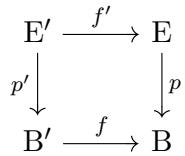
\includegraphics[keepaspectratio]{images/part003_c1a9b5e7.jpg}}

a Cartesian square. We assume that the map f is proper, separated, and surjective, and we make one of the following hypotheses:

\begin{enumerate}
\def\labelenumi{(\roman{enumi})}
\item
  The fibers of f are locally connected and the fibered square \(B^{\prime} \times_{B} B^{\prime}\) is locally connected.
\item
  The fibers of \(f\) are finite, the diagonal \(\Delta_{\mathrm{B}^{\prime}}\) of \(\mathrm{B}^{\prime}\times_{\mathrm{B}}\mathrm{B}^{\prime}\) is open in \(\mathrm{B}^{\prime}\times_{\mathrm{B}}\mathrm{B}^{\prime}\) and \(\mathrm{B}^{\prime}\times_{\mathrm{B}}\mathrm{B}^{\prime} - \Delta_{\mathrm{B}^{\prime}}\) is a locally connected space.
\end{enumerate}

Then, if \((\mathrm{E}^{\prime}, p^{\prime})\) is a covering, \((\mathrm{E}, p)\) is a covering.

Since the map \(f\) is universally strict (I, p.~20, corollary), the map \(p\) is étale (I, p.~31, prop. 8) and separated (I, p.~27, prop. 4). We shall assume, as is permissible, that \(\mathrm{E}' = \mathrm{B}' \times_{\mathrm{B}} \mathrm{E}\) .

Let \(a\) be a point of B; the aim is to show that the point \(a\) has a neighborhood W such that the W-space \((\mathrm{E_W}, p_{\mathrm{W}})\) is a trivializable covering. Set \(\mathrm{B}_a^\prime = f^{-1}(a)\) and set \(\mathrm{E}_a^\prime = (p')^{-1}(\mathrm{E}_a)\) . The map \(t_a: \mathrm{E}_a^\prime \to \mathrm{B}_a^\prime \times \mathrm{E}_a\) defined by \(t_a(y) = (p'(y), f'(y))\) is a \(\mathrm{B}_a^\prime\) -isomorphism (I, p.~9, prop. 4), hence \(\mathrm{E}_a^\prime\) is a trivializable covering of \(\mathrm{B}_a^\prime\) and \(t_a\) is a trivialization of this covering.

Let us prove that there exists a neighborhood \(V'\) of \(B'_{a}\) in \(B'\) and a continuous trivialization t of the covering ( \(E_{V'}', p_{V'}\) ) that extends \(t_{a}\) . Under hypothesis (ii), \(B'_{a}\) is finite and its points possess pairwise disjoint open neighborhoods over which the covering \(E'\) is trivializable, whence the assertion in this case. Under hypothesis (i), \(B'_{a}\) is locally connected, as is B' (IV, p.~390, lemma 1); since the map f is proper and separated, \(B'_{a}\) is compact and two distinct points have disjoint neighborhoods in B', so that the pair (B', \(B'_{a}\)) satisfies property (PCV) (I, p.~37, lemma 1). The assertion therefore follows from cor. 2 of I, p.~90.

Since \(f\) is proper, there exists a neighborhood \(V\) of \(a\) in \(B\) such that \(V'\) contains \(f^{-1}(V)\) (lemma, I, p.~75). One may thus assume that \(V' = f^{-1}(V)\) .

Equip the \(V'\)-spaces \(V' \times E_{a}\) and \(E_{V'}' = V' \times_{B} E\) with their canonical descent data relative to \(f_{V}: V' \to V\) . We shall show that, after possibly shrinking V and \(V'\), the isomorphism of \(V'\)-spaces \(t: E_{V'}' \to V' \times E_{a}\) that we have just defined is compatible with the descent data, that is, we have \(t(b_{1}', x) = t(b_{2}', x)\) if \((b_{1}', b_{2}') \in V' \times_{V} V'\) and \(x \in E_{f(b_{1}')}\) . Denote by \(\widetilde{t}\) the map \(pr_{2} \circ t: E_{V'}' \to E_{a}\) .

Let us set \(V'' = V' \times_{V} V'\) ; consider it as a \(V'\)-space by means of the first projection. The map \(((b_{1}', b_{2}'), x) \mapsto ((b_{1}', b_{2}'), (b_{1}', x))\) from \(V'' \times_{V} E\) into \(V'' \times_{V'} E'\) is an isomorphism of \(V''\)-spaces; this shows that \(V'' \times_{V} E\) is a covering of \(V''\) .

For \(i=1,2\) , we define a map \(u_{i}\colon V^{\prime\prime}\times_{V}E\to V^{\prime\prime}\times E_{a}\) by setting \(u_{i}(b_{1}^{\prime},b_{2}^{\prime},x)=(b_{1}^{\prime},b_{2}^{\prime},\widetilde{t}(b_{i}^{\prime},x))\) ; these are trivializations of the covering \(V^{\prime\prime}\times_{V}E\) . Let \(W^{\prime\prime}\) be the set of points \(w\in V^{\prime\prime}\) over which these trivializations \(u_{1}\) and \(u_{2}\) coincide; it contains \(B_{a}^{\prime}\times B_{a}^{\prime}\) , as well as the diagonal \(\Delta_{V'}\) . Let us prove that \(W^{\prime\prime}\) is a neighborhood of \(B_{a}^{\prime}\times B_{a}^{\prime}\) . Under hypothesis (i), this follows from cor. 2 of I, p.~80, since \(B^{\prime}\times B^{\prime}\) is locally connected. Under hypothesis (ii), \(W^{\prime\prime}\) contains a neighborhood of \((B_{a}^{\prime}\times B_{a}^{\prime})-\Delta_{B_{a}^{\prime}}\) in \((B^{\prime}\times_{B}B^{\prime})-\Delta_{B^{\prime}}\) , since this set is locally connected (loc. cit.). Since \(\Delta_{V'}\) is open in \(B^{\prime}\times_{B}B^{\prime}\) , \(W^{\prime\prime}\) is a neighborhood of \(B_{a}^{\prime}\times B_{a}^{\prime}\) in \(V^{\prime\prime}\) .

Since \(f\) is proper, the canonical map \(f''\) of \(\mathrm{B}' \times_{\mathrm{B}} \mathrm{B}'\) into B is proper, because it is the composite of the projection \(\mathrm{pr}_{1} \colon \mathrm{B}' \times_{\mathrm{B}} \mathrm{B}' \to \mathrm{B}'\) and of the mapping \(f\) .

By the lemma of I, p.~75, there exists a neighborhood W of a in V such that \((f'')^{-1}(\mathrm{W})\) is contained in \(W''\); set \(W'=(f')^{-1}(\mathrm{W})\), which is a subset of \(V'\) and the isomorphism of étale spaces \(t: E_{W'}' \to W' \times E_a\) is compatible with the canonical descent data relative to the map \(f_W: W' \to W\) . It follows from the corollary (IV, p.~388) that the

W-étale spaces \(E_{W}\) and \(W \times E_{a}\) are isomorphic. In particular, \(E_{W}\) is a trivializable covering, whence the proposition.

COROLLARY 1. --- Let E and B be topological spaces, \(p\colon\mathrm{E}\to\mathrm{B}\) a continuous map and \((\mathrm{A}_{i})_{i\in\mathrm{I}}\) a locally finite closed covering of B such that for every pair \((i,j)\in\mathrm{I}\times\mathrm{I}, i\neq j\) , the intersection \(\mathrm{A}_{i}\cap\mathrm{A}_{j}\) is a locally connected space. Then, for the B-space \((\mathrm{E},p)\) to be a covering, it is necessary and sufficient that, for every \(i\in\mathrm{I}\) , the \(\mathrm{A}_{i} \)-space \((p^{-1}(\mathrm{A}_{i}),p_{\mathrm{A}_{i}})\) be a covering of \(\mathrm{A}_{i}\) .

The condition is necessary (cf. I, p.~69). Conversely, let B' denote the topological sum space of the family \((\mathrm{A}_{i})_{i\in\mathrm{I}}\) and \(f\colon B'\to B\) the canonical map. The map f is closed (TG, I, p.~6, prop. 4), separated (I, p.~27, remark 5), with finite fibers, hence proper (TG, I, p.~75, th. 1); it is also surjective. The diagonal \(\Delta_{B'}\) , being equal to \(\bigcup_{i\in I}A_{i}\times_{B}A_{i}\) , is open in \(B'\times_{B}B'\) . Finally, the space \((\mathrm{B}'\times_{\mathrm{B}}\mathrm{B}')-\Delta_{\mathrm{B'}}\) is homeomorphic to the sum space of the family \((\mathrm{A}_{i}\cap\mathrm{A}_{j})\) , \((i,j)\in\mathrm{I}\times\mathrm{I}\) , \(i\neq j\) ; it is therefore locally connected. Hypothesis (ii) of proposition 6 is satisfied. If for every i, \(p^{-1}(\mathrm{A}_{i})\) is a covering of \(A_{i}\) , \(E'\) is then a covering of \(B'\) , hence E is a covering of B.

COROLLARY 2. --- Let X and Y be topological spaces and let \(f\colon X \to Y\) be a proper, separated, and surjective map. Moreover, assume one of the following hypotheses:

\begin{enumerate}
\def\labelenumi{(\roman{enumi})}
\item
  The fibers of f, as well as the space \(X\times_Y X\), are locally connected;
\item
  The fibers of \(f\) are finite, the diagonal \(\Delta_{\mathrm{X}}\) of \(\mathrm{X} \times_{\mathrm{Y}} \mathrm{X}\) is open in \(\mathrm{X} \times_{\mathrm{Y}} \mathrm{X}\) and the space \((\mathrm{X} \times_{\mathrm{Y}} \mathrm{X}) - \Delta_{\mathrm{X}}\) is locally connected. Then, every descent datum relative to \(f\) on a covering of \(\mathrm{X}\) is effective, and the quotient space is a covering of \(\mathrm{Y}\) .
\end{enumerate}

Let Z be a covering of X and let \(\tau\) be a descent datum relative to f on Z. By proposition 5 (IV, p.~389), the descent datum \(\tau\) is effective, in other words the square

\pandocbounded{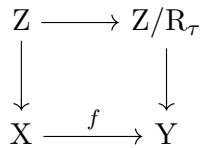
\includegraphics[keepaspectratio]{images/part003_fd3d7e4d.jpg}}

is a Cartesian square. The hypotheses of proposition 6 (IV, p.~391) are then satisfied. Consequently, \(Z/R_{\tau}\) is a covering of Y.

PROPOSITION 7. --- Let X and Y be topological spaces and let \(f: X \to Y\) be a continuous and surjective map. Suppose that Y is deloopable and that the map f is open and has the path-lifting property. Then, every descent datum relative to f on a covering of X is effective, and the quotient space is a covering of Y.

Let \((Z,p)\) be a covering of X and let \(\tau\) be a descent datum relative to f on Z. Since the map f is surjective and open, it follows from prop. 5 of IV, p.~389, that the descent datum \(\tau\) is effective. Let \(T = Y/R_{\tau}\) denote the quotient Y-space; its projection q is étale (loc. cit.), and it is also separated (I, p.~27, prop. 4).

By hypothesis, the map f has the path lifting property, as does the map p, since Z is a covering of X (III, p.~302, corollary 2 of prop. 3). Consequently, the same holds for the map \(p \circ f\) , hence for the map q. Therefore (cf.~IV, p.~341, remark 2), T is a covering of Y. The proposition is thus proved.

Remark. --- Let X and Y be topological spaces and let \(f: X \rightarrow Y\) be a map. For every descent datum relative to f on a covering of X to be effective, and for the quotient space to be a covering of Y, it is necessary that f be strict and that \(f(X)\) be an open and closed subset of X.

Indeed, identify the X-space X with \(X \times_{Y} Y\) and endow it with its canonical descent datum relative to f. The quotient space is identified with \(f(\mathrm{X})\) , equipped with the quotient topology of the topology of X for the equivalence relation defined by f. If this is a covering of Y, the space \(f(\mathrm{X})\) is then identified with an open and closed subset of Y and the map f is strict.

\subsection{Descent of groupoids}

Let X and Y be topological spaces, and let \(f\colon\mathrm{X}\to\mathrm{Y}\) be a continuous map. Let \(p_{1}\) and \(p_{2}\) be the two projections of \(\mathrm{X}\times_{\mathrm{Y}}\mathrm{X}\) into X, \(\operatorname{Coeg}(f)\) the coequalizer groupoid of the pair \((\varpi(p_{1}),\varpi(p_{2}))\) of groupoid morphisms from \(\varpi(\mathrm{X}\times_{\mathrm{Y}}\mathrm{X})\) into \(\varpi(\mathrm{X})\), and \(\gamma\colon\varpi(\mathrm{X})\to\operatorname{Coeg}(f)\) the canonical groupoid morphism (II, p.~199, def. 2). Since \(f\circ p_{1}=f\circ p_{2}\) , we have \(\varpi(f)\circ\varpi(p_{1})=\varpi(f)\circ\varpi(p_{2})\) . It then follows from the universal property of coequalizers (II, p.~199, prop. 3) that there exists a unique morphism of groupoids \(\varpi'(f)\colon\operatorname{Coeg}(f)\to\varpi(\mathrm{Y})\) such that \(\varpi(f)=\varpi'(f)\circ\gamma\) .

The set of vertices of Coeg(f) is the quotient set of the set X = Vert( \(\varpi(X)\) ) by the equivalence relation defined by f (II, p.~200, remark 1). It is identified with f(X).

PROPOSITION 8. --- Let X and Y be nonempty topological spaces and let f be a continuous map from X to Y. Suppose that X is locally path-connected, Y is connected, and f is strict and surjective. Then the groupoid Coeg(f) is transitive.

Let \(\Gamma\) be the quiver whose set of vertices is X and whose set of arrows is the disjoint union of \(\mathrm{Fl}(\varpi(\mathrm{X}))\) and \(\mathrm{X}\times_{\mathrm{Y}}\mathrm{X}\), the source and target maps being those of \(\varpi(\mathrm{X})\) on \(\mathrm{Fl}(\varpi(\mathrm{X}))\) and the maps \(p_1\) and \(p_2\) on \(\mathrm{X}\times_{\mathrm{Y}}\mathrm{X}\) . By the definition of the frame of the pair \((\varpi(\mathrm{pr}_1), \varpi(\mathrm{pr}_2))\) (II, p.~185, def. 3) and remark 2 of II, p.~200, the set of orbits of \(\operatorname{Coeg}(f)\) is identified with the set of connected components of the quiver \(\Gamma\) . Since the space X is not empty, it suffices to prove that the graph \(\Gamma\) is connected.

The connected components of \(\Gamma\) are saturated for the equivalence relation “there exists a path joining \(x\) to \(x'\) ”, hence are open in X, because X is locally path-connected. They are then also closed. They are also saturated for the equivalence relation R defined by f . By hypothesis, the map f induces a homeomorphism from X/R onto Y, so that the image under f of every connected component of \(\Gamma\) is an open and closed subset of Y, hence is equal to Y since the space Y is assumed to be connected.

Let C be a connected component of \(\Gamma\) , let \(x\) be a point of X. By the preceding, there exists a point \(x' \in \mathrm{C}\) such that \(f(x') = f(x)\) . By definition of the quiver \(\Gamma\) , we have \(x' \in \mathrm{C}\) . One thus has \(\mathrm{C} = \mathrm{X}\) and the quiver \(\Gamma\) is therefore connected.

PROPOSITION 9. --- Let X and Y be topological spaces and let f be a continuous map from X to Y. Suppose that the space X is locally path-connected, that the space Y is deloopable, and that the map f is strict and surjective. Then, the groupoid \(\varpi(\mathrm{Y})\) is generated by the image of \(\varpi(\mathrm{X})\) under \(\varpi(f)\) .

We may assume that the spaces X and Y are nonempty. Let G denote the subgroupoid of \(\varpi(\mathrm{Y})\) generated by the image of \(\varpi(\mathrm{X})\) under \(\varpi(f)\) . As the map f is surjective, the set of vertices of G is equal to Y. By prop. 8, \(\operatorname{Coeg}(f)\) is a transitive groupoid. Since \(\varpi'(f)\) induces the identity on the vertices, the image of \(\operatorname{Coeg}(f)\) under \(\varpi'(f)\) is a transitive subgroupoid of \(\varpi(\mathrm{Y})\) . The image of \(\varpi(\mathrm{X})\) under \(\gamma\) generates \(\operatorname{Coeg}(f)\) (II, p.~200, corollary); since we have \(\varpi(f) = \varpi'(f) \circ \gamma\) , the groupoid G is transitive.

Let \(y_{0}\) be a point of Y and let H denote the subgroup \(G_{y_{0}}\) of \(\pi_{1}(Y, y_{0})\) . By th. 1 of IV, p.~342, there exists a connected covering (T, p) of Y and a point \(t_{0}\) of the fiber \(T_{y_{0}}\) whose fixator is H.

If \(x\) is a point of X, the set \(\mathrm{Fl}_{y_0,f(x)}(\mathrm{G})\) is nonempty, since G is transitive. For \(u\in \mathrm{Fl}_{y_0,f(x)}(\mathrm{G})\) , the point \(t_0\cdot u\) is a point of the fiber \(\mathrm{T}_{f(x)}\) , independent of \(u\) since the group H, the isotropy group of G at \(y_0\) , fixes \(t_0\) . Denote by \(\sigma (x)\) this point; denote by \(\sigma \colon \mathrm{X}\to \mathrm{T}\) the map thus defined and \(s\colon \mathrm{X}\to \mathrm{X}\times_{\mathrm{Y}}\mathrm{T}\) the map \(x\mapsto (x,\sigma (x))\) . By construction, the map s is compatible with the canonical actions of \(\varpi (\mathrm{X})\) on X and \(\mathrm{X}\times_{\mathrm{Y}}\mathrm{T}\) . It then follows from Lemma 1 of III, p.~312, that s is continuous. The map \(\sigma\) is therefore continuous; moreover, it is compatible with the equivalence relation defined by f since \(\sigma (x)\) depends only on \(f(x)\) . Since f is strict and surjective, there exists a unique continuous map \(\overline{\sigma}\colon \mathrm{Y}\to \mathrm{T}\) such that \(\overline{\sigma}\circ f = \sigma\) , so that the covering T admits a section. Since T is connected, the map \(p\colon \mathrm{T}\to \mathrm{Y}\) is a homeomorphism (I, p.~31, cor. 4 of prop. 6) and one has \(\mathrm{H} = \pi_1(\mathrm{Y},y_0)\) , whence \(\mathrm{G}_{y_0} = \pi_1(\mathrm{Y},y_0)\) . Since G is transitive, it follows that \(\mathrm{G} = \varpi (\mathrm{Y})\) .

PROPOSITION 10. --- Let X and Y be topological spaces and let f be a continuous map from X to Y. Suppose that the space X is deloopable, that the space \(X\times_{Y}X\) is locally path-connected, and that every descent datum relative to f on a covering of X is effective and the quotient space is a covering of Y. Then, the groupoid morphism \(\varpi'(f)\) from Coeg(f) into \(\varpi(Y)\) is injective.

Under the hypotheses of the proposition, \(f\) is strict (IV, p.~394, remark); one may moreover assume that it is surjective.

Lemma 2. --- Keep the notations and hypotheses of the proposition. Let T be a set equipped with an action of the groupoid Coeg(f) relative to a map q: T → Y. Then there exists a unique topology on T for which q makes T a covering of Y such that for every path class with origin c in X and every point t in T, one has \(t \cdot \gamma(c) = t \cdot f_{*}(c)\) . In particular, the action of Coeg(f) on T factors through an action of the groupoid \(\varpi(Y)\) .

The uniqueness of such a topology on T follows from Lemma 1 (III, p.~312); let us prove its existence. Endow the set \(X\times_{Y}T\) with an action of \(\varpi(\mathrm{X})\) by setting \((x,t)\cdot u=(x\cdot u,t\cdot\gamma(u))\) for all \((x,t)\in\mathrm{X}\times_{\mathrm{Y}}\mathrm{T}\) and every arrow u with source x in \(\varpi(\mathrm{X})\). Since the space X is deloopable, this action is without local monodromy (III, p.~313, remark). There therefore exists on the set \(X\times_{Y}T\) a unique topology that makes the X-space \((\mathrm{X}\times_{\mathrm{Y}}\mathrm{T},\mathrm{pr}_{1})\) a covering of X such that the canonical action of \(\varpi(\mathrm{X})\) on this covering coincides with the given action (III, p.~313, prop. 3). Let us denote this covering by \((Z,p)\). Let us show that the map \(\tau: ((x_{1},t),x_{2})\mapsto(x_{2},t)\) from \(Z\times_{Y}X\) into Z is a descent datum on Z relative to the map f. It suffices to verify that it is continuous, the other conditions of Definition 1 of IV, p.~382, being evident.

The map \(\tau\) is a lifting of the map \(\mathrm{pr}_2\colon Z\times_Y X\to X\) to the covering \(Z\) of \(X\) . Since the space \(X\times_Y X\) is locally path-connected, the space \(Z\times_Y X\) , which is a covering of it, is also locally path-connected. By the corollary (III, p.~269), to show that the map \(\tau\) is continuous, it suffices to show that it is continuous by paths.

So let \(\widetilde{c} = ((c,g),c')\) be a path in \(Z\times_{Y}X\) and let us show that the map \(\tau \circ \widetilde{c}\colon t\mapsto (c'(t),g(t))\) from I to Z is continuous. For every \(s\in [0,1]\) , denote by \(c_s\) and \(c_s'\) the paths in X defined by \(t\mapsto c(st)\) and \(t\mapsto c'(st)\) . For all \(s\in [0,1]\) , we thus have \(c(s) = c(0)\cdot [c_s]\) , \(c'(s) = c'(0)\cdot [c_s']\) and \((c,g)(s) = (c(0),g(0))\cdot [c_s]\) , where \([u]\) denotes the strict homotopy class of a path u (III, p.~304, remark). The map \(t\mapsto (c_s(t),c_s'(t))\) is a path in \(X\times_{Y}X\) ; by definition of the coequalizer Coeg(f), we therefore have \(\gamma ([c_s]) = \gamma ([c_s'])\) and \(g(s) = g(0)\cdot \gamma ([c_s]) = g(0)\cdot \gamma ([c_s'])\) . By definition of the action of \(\varpi (X)\) on Z, we therefore have

\[
\begin{array}{r} (\tau \circ \widetilde {c}) (s) = (c ^ {\prime} (s), g (s)) = (c ^ {\prime} (0) \cdot [ c _ {s} ^ {\prime} ], g (0) \cdot \gamma ([ c _ {s} ^ {\prime} ])) \\ = (c ^ {\prime} (0), g (0)) \cdot [ c _ {s} ^ {\prime} ] = (\tau \circ \widetilde {c}) (0) \cdot [ c _ {s} ^ {\prime} ]. \end{array}
\]

This shows that \(\tau \circ \widetilde{c}\) is a continuous lift to Z of the path \(c'\) (loc. cit.). Consequently, the map \(\tau\) is continuous by paths, hence continuous; it is a descent datum relative to \(f\) on the X-space Z.

Denote by \(R_{\tau}\) the equivalence relation defined by the descent datum \(\tau\) . Since the map f is surjective, the map \(pr_{2}: Z \to T\) induces, by passing to the quotient, a bijection from \(Z/R_{\tau}\) onto T. Endow T with the topology deduced from that of \(Z/R_{\tau}\) by transport of structure, so that \((T,q)\) is a Y-space. By hypothesis, T is therefore a covering of Y and the diagram

\[
\begin{array}{c} \mathrm{Z} \xrightarrow {\mathrm{pr} _ {2}} \mathrm{T} \\ p \Big \downarrow \qquad \qquad \qquad \qquad \Big \downarrow q \\ \mathrm{X} \xrightarrow {f} \mathrm{Y} \end{array}
\]

is a Cartesian square.

Let \((x,t)\) be a point of Z, let c be a path with origin x in X, and let \(\widetilde{c}\) be the continuous lift of c to Z with origin \((x,t)\) . The path \(pr_{2} \circ \widetilde{c}\) is the lift with origin t of the path \(f \circ c\) of Y, so that \(t \cdot \gamma([c]) = t \cdot [f \circ c] = t \cdot f_{*}([c])\) . This concludes the proof of the lemma.

Let us now prove the proposition. Let \(u\) and \(v\) be two arrows of Coeg( \(f\) ) whose images in \(\varpi(Y)\) are equal. The groupoid morphism \(\varpi'(f)\) being the identity on the vertex sets, the arrows \(u\) and \(v\) have the same origin and the same target. Let us denote by \(y\) the origin of \(u\) ; let T be the set of arrows of Coeg( \(f\) ) with source y and let \(q: \mathrm{T} \to \mathrm{Y}\) the restriction to T of the target map. The groupoid Coeg( \(f\) ) acts by right composition on the set T, relative to \(q\) . By Lemma 2, the actions of \(u\) and \(v\) on T are identical. We therefore have \(u = e_y \cdot u = e_y \cdot v = v\) . This proves that the groupoid morphism \(\varpi'(f)\) is injective.

THEOREM 1. --- Let X and Y be topological spaces, let \(f: X \to Y\) be a continuous and surjective map. Suppose the spaces X and Y are deloopable. Finally, suppose that one of the following properties is satisfied:

\begin{enumerate}
\def\labelenumi{(\roman{enumi})}
\item
  The map f is proper, separated, with locally connected fibers, and the space \(X\times_{Y}X\) is locally path-connected;
\item
  The map f is proper, separated, with finite fibers, the diagonal \(\Delta_{X}\) is open in \(X \times_{Y} X\) and its complement is locally connected;
\item
  The map f is open and has the path lifting property.
\end{enumerate}

Then, the morphism of groupoids \(\varpi'(f)\) is an isomorphism from the groupoid Coeg(f) onto the Poincaré groupoid \(\varpi(Y)\) .

Let us first note that under these hypotheses, the map \(f\) is surjective and strict (I, p.~18, example 2). Moreover, every descent datum relative to \(f\) on a covering of X is effective, and the quotient space is a covering of Y; this follows from IV, p.~393, corollary 2 of prop. 4 under hypotheses (i) and (ii), and from prop. 7 of IV, p.~394 under hypothesis (iii). By prop. 10, the morphism of groupoids \(\varpi'(f)\) is therefore injective, and its image is a subgroupoid of \(\varpi(Y)\) .

By prop. 9 of IV, p.~395, this image is equal to \(\varpi(\mathrm{Y})\) under hypotheses (i) and (ii), but also under hypothesis (iii) since the groupoid morphism \(\varpi(f)\) is then surjective.

Therefore, \(\varpi'(f)\) is an isomorphism.

Examples. --- Here are two examples where the hypotheses of Theorem 1 are satisfied.

\begin{enumerate}
\def\labelenumi{\arabic{enumi})}
\item
  Let Y be a deloopable topological space. Let \((\mathrm{A}_{i})_{i\in\mathrm{I}}\) be a locally finite cover of Y by closed sets. Suppose that, for every \(i\in I\) , the space \(A_{i}\) is deloopable and that, for every pair \((i,j)\in\mathrm{I}\times\mathrm{I}\) , the space \(A_{i}\cap A_{j}\) is locally path-connected. One may take for X the sum space of the family \((\mathrm{A}_{i})_{i\in\mathrm{I}}\) and for \(f:X\to Y\) the map deduced from the family of canonical injections.
\item
  Let G be a discrete group acting properly on a deloopable topological space X; set Y = X/G and let \(f: X \to Y\) be the canonical map. It is open (TG, III, p.~10, lemma 2) and has the path-lifting property by virtue of Theorem 4 of III, p.~287. The space Y is deloopable according to IV, p.~349, prop. 8, b). By hypothesis, the map from G × X to \(X\times X\) given by \((g, x) \mapsto (g \cdot x, x)\) is proper, hence strict (I, p.~18, example 2), and its image is \(X\times_{Y}X\). It then follows from III, p.~261, prop. 8 that \(X\times_{Y}X\) is locally path-connected.
\end{enumerate}

\subsection{Descent by an étale and surjective map}

Let X and Y be topological spaces, and let f be a continuous map from X to Y. We retain the notation of the preceding section.

THEOREM 2. --- Suppose that every point of Y has a neighborhood over which there exists a continuous section of the map f. Then the groupoid morphism \(\varpi'(f)\) from \(\operatorname{Coeg}(f)\) into \(\varpi(Y)\) is an isomorphism.

By hypothesis, there exists a covering \((\mathrm{U}_{j})_{j\in\mathrm{J}}\) of Y by open sets and, for every \(j\in J\), a continuous section \(s_{j}\) of \(f_{U_{j}}\) .

If \(c\) is a path in X, we will denote by \([c]\) its strict homotopy class in \(\varpi(X)\) and by \(\{c\}\) the image of \([c]\) in \(\operatorname{Coeg}(f)\) under the groupoid morphism \(\gamma\) . If \(c\) and \(c'\) are two paths in X, \(\{c\}\) and \(\{c'\}\) are composable in \(\operatorname{Coeg}(f)\) if and only if the paths \(f \circ c\) and \(f \circ c'\) in Y are juxtaposable.

Let \(c'\) be a path in Y. By Lemma 4 of III, p.~272, applied to the compact space I and the covering \(((c')^{-1}(\mathrm{U}_j))_{j\in \mathrm{J}}\) of I, there exists an integer \(n\) such that, for every integer \(k\) satisfying \(1\leqslant k\leqslant n\), the image of the interval \([\frac{k - 1}{n},\frac{k}{n}]\) under \(c'\) is contained in an open set \(\mathrm{U}_{j(k)}\) . For every integer \(k\) , \(1\leqslant k\leqslant n\) , let \(c_k'\) be the path in Y defined by \(s\mapsto c'(\frac{k + s - 1}{n})\) ; we have \([c'] = [c_1'][c_2']\ldots [c_n']\) (cf. III, p.~291, Remark 1), and \(c'\) is the path denoted \(c_1' * c_2' * \dots * c_n'\) . For all \(k\in \{1,\ldots ,n\}\) , denote by \(c_k\) the path \(s_{j(k)}\circ c_k'\) in X and set \(\{c_k\} = \gamma ([c_k])\) . Since for every \(k\) the paths \(c_{k - 1}' = f\circ c_{k - 1}\) and \(c_k' = f\circ c_k\) are juxtaposable, the sequence \((\{c_1\} ,\ldots ,\{c_n\})\) is composable in \(\operatorname{Coeg}(f)\). By construction,

\[
\begin{array}{r l} & {\varpi^ {\prime} (f) (\{c _ {1} \} \ldots \{c _ {n} \}) = \varpi^ {\prime} (f) (\{c _ {1} \}) \ldots \varpi^ {\prime} (f) (\{c _ {n} \})} \\ & {\qquad = \varpi (f) ([ c _ {1} ]) \ldots \varpi (f) ([ c _ {n} ])} \\ & {\qquad = [ f \circ c _ {1} ] \ldots [ f \circ c _ {n} ]} \\ & {\qquad = [ c _ {1} ^ {\prime} ] * \dots * [ c _ {n} ^ {\prime} ] = [ c ^ {\prime} ],} \end{array}
\]

which proves that the groupoid morphism \(\varpi'(f)\) is surjective.

Let \(u\) and \(v\) be arrows of \(\operatorname{Coeg}(f)\) . Since the groupoid \(\operatorname{Coeg}(f)\) is generated by the image of \(\varpi(\mathrm{X})\) (II, p.~200, corollary), there exist finite sequences \((c_1, \ldots, c_n)\) and \((d_1, \ldots, d_n)\) of paths in X such that one has \(u = \{c_1\} \ldots \{c_n\}\) and \(v = \{d_1\} \ldots \{d_n\}\) . The paths \((f \circ c_1, \ldots, f \circ c_n)\) in Y are then juxtaposable and one has \(\varpi'(f)(u) = [(f \circ c_1)] \ldots [(f \circ c_n)]\) ; likewise, \(\varpi'(f)(v) = [(f \circ d_1)] \ldots [(f \circ d_n)]\) .

Suppose that we have \(\varpi'(f)(u) = \varpi'(f)(v)\) . There then exists a strict homotopy \(\sigma\) connecting \((f \circ c_1) * \cdots * (f \circ c_n)\) to \((f \circ d_1) * \cdots * (f \circ d_n)\) . By Lemma 4 of III, p.~272, applied to the compact space \(\mathbf{I} \times \mathbf{I}\) and the covering \((\bar{\sigma}^{-1}(\mathrm{U}_i))_{i \in \mathrm{I}}\) of \(\mathbf{I} \times \mathbf{I}\) , there exists an integer \(m \geqslant 1\) such that, for every pair of integers \((j,k)\) satisfying \(1 \leqslant j \leqslant m\) and \(1 \leqslant k \leqslant m\), the image of \([\frac{j-1}{m}, \frac{j}{m}] \times [\frac{k-1}{m}, \frac{k}{m}]\) under \(\sigma\) is contained in an open set \(U_{i(j,k)}\) of the covering \((\mathrm{U}_{i})_{i \in \mathrm{I}}\) .

Every path c in X is of the form \(c_{1}*\cdots*c_{m}\) , where \(c_{k}\) is the path \(t\mapsto c(\frac{k-1+t}{m})\) . If necessary, replacing the integers m and n by their product mn, one may therefore suppose that m=n.

For every pair \((j,k)\) of integers of \(\{1,\ldots ,n\}\) and every pair \((s,t)\in\) \(\mathbf{I}\times \mathbf{I}\) , set

\[
\sigma_ {j, k} (s, t) = s _ {i (j, k)} \circ \sigma \left(\frac {s + j - 1}{n}, \frac {t + k - 1}{n}\right).
\]

For \(t \in \mathbf{I}\) , also set \(h_{j,k}^{0}(t) = \sigma_{j,k}(t,0)\) , \(h_{j,k}^{1}(t) = \sigma_{j,k}(t,1)\) , \(v_{j,k}^{0}(t) = \sigma_{j,k}(0,t)\) and \(v_{j,k}^{1}(t) = \sigma_{j,k}(1,t)\) . By Lemma 1 of III, p.~295, the paths \(h_{j,k}^{0} * v_{j,k}^{1}\) and \(v_{j,k}^{0} * h_{j,k}^{1}\) are strictly homotopic, whence the relation

\[
[ h _ {j, k} ^ {0} ] [ v _ {j, k} ^ {1} ] = [ v _ {j, k} ^ {0} ] [ h _ {j, k} ^ {1} ]\tag{2}
\]

on \(\varpi(\mathrm{X})\) , for every pair \((j,k) \in \{1, \ldots, n\}^2\) . On the other hand, for every pair of integers \((j,k)\) , with \(2 \leqslant j \leqslant n\) and \(1 \leqslant k \leqslant n\) , we have \(f \circ v_{j,k}^0 = f \circ v_{j-1,k}^1\) , whence the relation

\[
\{v _ {j, k} ^ {0} \} = \{v _ {j - 1, k} ^ {1} \}\tag{3}
\]

in Coeg(f). Likewise, for every pair of integers \((j,k)\) such that \(1 \leqslant j \leqslant n\) and \(2 \leqslant k \leqslant n\) , we have

\[
\{h _ {j, k} ^ {0} \} = \{h _ {j, k - 1} ^ {1} \}.\tag{4}
\]

For \(j \in \{1, \ldots, n\}\) the paths \(f \circ c_j\) and \(f \circ h_{j,1}^0\) coincide. By definition of the coequalizer Coeg(f), one therefore has \(\{c_j\} = \{h_{j,1}^0\}\) . Likewise, for every \(j \in \{1, \ldots, n\}\) , \(\{d_j\} = \{h_{j,n}^1\}\) . Consequently, one has the relations

\[
u = \{h _ {1, 1} ^ {0} \} \dots \{h _ {n, 1} ^ {0} \}, \quad v = \{h _ {1, n} ^ {1} \} \dots \{h _ {n, n} ^ {1} \}.
\]

By Lemma 3 below, one has

\[
\{h _ {1, 1} ^ {0} \} \dots \{h _ {1, n} ^ {0} \} \{v _ {1, n} ^ {1} \} \dots \{v _ {n, n} ^ {1} \} = \{v _ {1, 1} ^ {0} \} \dots \{v _ {n, 1} ^ {0} \} \{h _ {n, 1} ^ {1} \} \dots \{h _ {n, n} ^ {1} \}.
\]

Since the paths \(t \mapsto \sigma(0,t)\) and \(t \mapsto \sigma(1,t)\) are constant, one has, for \(1 \leqslant k \leqslant n\) , \(\{v_{1,k}^{0}\} = e_{a}\) and \(\{v_{n,k}^{1}\} = e_{b}\) where \(a,b \in Y\) are the source and the target of the arrows \(u\) and \(v\) of Coeg( \(f\) ). It follows that one has the equality

\[
\{h _ {1, 1} ^ {0} \} \dots \{h _ {1, n} ^ {0} \} = \{h _ {n, 1} ^ {0} \} \dots \{h _ {n, n} ^ {1} \},
\]

that is, u = v.

Lemma 3. --- Let G be a groupoid and let p, q be integers \(\geqslant 1\) . For every pair \((j, k)\) of integers such that \(0 \leqslant j \leqslant p\) and \(0 \leqslant k \leqslant q\) , let \(x_{j,k}\) be a vertex of G; for every pair \((j, k)\) such that \(1 \leqslant j \leqslant p\) and \(0 \leqslant k \leqslant q\) , let \(h_{j,k}\) be an arrow of G connecting \(x_{j-1,k}\) to \(x_{j,k}\) ; for every pair \((j, k)\) such that \(0 \leqslant j \leqslant p\) and \(1 \leqslant k \leqslant q\) , let \(v_{j,k}\) be an arrow of G connecting \(x_{j,k-1}\) to \(x_{j,k}\) .

Suppose that, for every pair \((j,k)\) of integers such that \(1 \leqslant j \leqslant p\) and \(1 \leqslant k \leqslant q\) , the arrows \(v_{j-1,k}\) and \(h_{j,k}\) are composable, as are the arrows \(h_{j,k-1}\) and \(v_{j,k}\) , and that one has \(v_{j-1,k}h_{j,k} = h_{j,k-1}v_{j,k}\) . Then,

\[
h _ {1, 0} h _ {2, 0} \dots h _ {p, 0} v _ {p, 1} v _ {p, 2} \dots v _ {p, q} = v _ {0, 1} v _ {0, 2} \dots v _ {0, q} h _ {1, q} h _ {2, q} \dots h _ {p, q}.
\]

First treat the particular case where q = 1 and prove the result by induction on p. If p = 1, the assertion to be proved is verified by hypothesis; suppose it is verified for p - 1; one then has

\[
h _ {1, 0} h _ {2, 0} \dots h _ {p, 0} v _ {p, 1} = h _ {1, 0} h _ {2, 0} \dots h _ {p - 1, 0} v _ {p - 1, 1} h _ {p, 1} = v _ {0, 1} h _ {1, 1} \dots h _ {p, 1}
\]

by the induction hypothesis, whence the relation for p.

Now prove the result by induction on q. It is true for q = 1 by what precedes; if it is true for q - 1, one then has

\[
h _ {1, 0} h _ {2, 0} \dots h _ {p, 0} v _ {p, 1} v _ {p, 2} \dots v _ {p, q} = v _ {0, 1} v _ {0, 2} \dots v _ {0, q - 1} h _ {1, q - 1} \dots h _ {p, q - 1} v _ {p, q}.
\]

By the case \(q = 1\) , we have

\[
h _ {1, q - 1} \dots h _ {p, q - 1} v _ {p, q} = v _ {0, q} h _ {1, q} \dots h _ {p, q},
\]

whence the desired relation.

Examples. --- 1) The theorem applies when the map f is étale and surjective.

\begin{enumerate}
\def\labelenumi{\arabic{enumi})}
\setcounter{enumi}{1}
\tightlist
\item
  It also applies when the space X is the sum space of a family \((V_{i})_{i\in\mathrm{I}}\) of subsets of Y whose interiors cover Y, and f is the map deduced from the canonical injections of each of the \(V_{i}\) in Y.
\end{enumerate}

\subsection{Poincaré groupoid of a quotient space}

Let X be a topological space equipped with a continuous action of a discrete group G; set Y = X/G and denote by \(f: X \to Y\) the canonical map. Denote by \(\lvert G\rvert\) the groupoid \(\varpi(G)\); its set of vertices is G; for \(g, g' \in G\) , there exists a unique arrow from g to \(g'\) if \(g' = g\) and none otherwise. By passing to fundamental groupoids, the operation \(m: G \times X \to X\) induces a morphism of groupoids \(\varpi(m): \lvert G\rvert \times \varpi(X) \to \varpi(X)\) . Let \(\varpi(X)/G\) be the coequalizer of the two morphisms of groupoids \(\varpi(m)\) and \(\varpi(\mathrm{pr}_{2})\) of \(\lvert G\rvert \times \varpi(X)\) into \(\varpi(X)\) ; let us denote by \(\beta: \varpi(X) \to \varpi(X)/G\) the canonical morphism of groupoids. We have \(f \circ m = f \circ pr_{2}\) , therefore \(\varpi(f) \circ \varpi(m) = \varpi(f) \circ \varpi(\mathrm{pr}_{2})\) . By the universal property of coequalizers, there therefore exists a unique morphism of groupoids \(\varpi''(f): \varpi(X)/G \to \varpi(Y)\) such that one has \(\varpi(f) = \varpi''(f) \circ \beta\) .

THEOREM 3. --- Let X be a deloopable topological space and let G be a discrete group acting properly on X; let \(f\colon X \to X/G\) be the canonical surjection. The canonical groupoid morphism \(\varpi''(f)\colon \varpi(X)/G \to \varpi(X/G)\) introduced above is an isomorphism.

Denote by \(\operatorname{Coeg}(f)\) the coequalizer of the two groupoid morphisms from \(\varpi(\mathrm{X} \times_{\mathrm{Y}} \mathrm{X})\) into \(\varpi(\mathrm{X})\) induced by the projections \(pr_{1}\) and \(pr_{2}\) ; let \(\gamma: \varpi(\mathrm{X}) \to \operatorname{Coeg}(f)\) be the canonical groupoid morphism. The image of the map \((m, pr_{2})\) : \(G \times X \to X \times X\) being the subspace \(X \times_{Y} X\) of \(X \times X\) , the two groupoid morphisms \(\gamma \circ \varpi(m)\) and \(\gamma \circ \varpi(pr_{2})\) of \(\lvert G\rvert \times \varpi(X)\) into \(\operatorname{Coeg}(f)\) are equal. By the universal property of \(\varpi(\mathrm{X})/\mathrm{G}\) , there exists a unique morphism of groupoids \(\alpha: \varpi(\mathrm{X})/\mathrm{G} \to \operatorname{Coeg}(f)\) such that \(\gamma = \alpha \circ \beta\) .

We also denote by \(\varpi'(f)\) the unique groupoid morphism from \(\operatorname{Coeg}(f)\) into \(\varpi(Y)\) such that \(\varpi(f) = \varpi'(f) \circ \gamma\) . By IV, p.~399, example 2, the hypotheses of th. 1 of IV, p.~398 are satisfied and the morphism \(\varpi'(f)\) is an isomorphism. Since

\[
\varpi (f) = \varpi^ {\prime} (f) \circ \gamma = \varpi^ {\prime} (f) \circ \alpha \circ \beta = \varpi^ {\prime \prime} (f) \circ \beta ,
\]

we have \(\varpi''(f) = \varpi'(f) \circ \alpha\) . Thus, to prove Theorem 3, it suffices to show that the morphism \(\alpha\) is an isomorphism.

Lemma 4. --- For every path \(c = (c_1, c_2)\) in \(X \times_Y X\) , we have \(\beta([c_1]) = \beta([c_2])\) .

Let c be such a path.

Let \(x \in X\) , let \(K_x\) be its stabilizer in G. By TG, III, p.~32, prop. 8, there exists an open neighborhood \(U_x\) of \(x\) in X such that \(K_x \cdot U_x = U_x\),

\(g \cdot U_x \cap U_x = \varnothing\) for all \(g \in G - K_x\) and such that the map f induces a homeomorphism from \(U_x/K_x\) onto an open neighborhood \(V_x\) of \(f(x)\) in Y. Since X is deloopable and the restriction to \(U_x\) of the map f is open and closed, one may moreover assume that \(U_x\) is connected and that the image of the canonical homomorphism \(\pi_1(U_x, x) \to \pi_1(X, x)\) is reduced to the identity element. The open sets \((V_x)_{x \in X}\) thus constructed form an open covering of Y. By Lemma 4 of III, p.~272, applied to the compact space I and the open sets \((f \circ c_1)^{-1}(V_x)\) for \(x \in X\) , there exists an integer \(n \geqslant 1\) such that for every \(i \in \{1, \ldots, n\}\) , there exists a point \(x_i\) in X such that \(c_1([i-1/n, i/n])\) is contained in \(f(V_{x_i})\) . Since \(f \circ c_1 = f \circ c_2\) , \(c_2([i-1/n, i/n])\) is also contained in \(f(V_{x_i})\) .

For \(j = 1\) or 2 and for \(i \in \{1, \ldots, n\}\) , denote by \(c_{j,i}\) the path in X defined by \(t \mapsto c_j(\frac{i+t-1}{n})\) ; we have \(c_j = c_{j,1} * \cdots * c_{j,n}\) (III, p.~291, remark 1). Consequently, to show that \(\beta([c_1]) = \beta([c_2])\) , it suffices to show that \(\beta([c_{1,i}]) = \beta([c_{2,i}])\) for every integer \(i \in \{1, \ldots, n\}\) . Replacing the path \((c_1, c_2)\) by the path \((c_{1,i}, c_{2,i})\) , we may thus assume that there exists \(x \in X\) such that \((f \circ c_1)([0,1]) \subset V_x\) .

The inverse image of \(V_{x}\) under f is the disjoint union of the connected components \(g \cdot U_{x}\) where g runs over a system of representatives in G of \(G/K_{x}\) . For i = 1 or 2, let \(g_{i}\) be an element of G such that the point \(x_{i} = g_{i} \cdot c_{i}(0)\) belongs to \(U_{x}\) . The image of the path \(g_{i} \cdot c_{i}\) is then contained in \(U_{x}\) . By definition of the groupoid \(\varpi(\mathrm{X})/\mathrm{G}\) , we have \(\beta([g_{i} \cdot c_{i}]) = \beta([c_{i}])\) which allows us to assume that the images of the paths \(c_{1}\) and \(c_{2}\) are contained in \(U_{x}\) and that \(g_{1} = g_{2} = e\) .

For \(s=0\) or 1, let \(d_{s}\) be a path in \(\mathrm{U}_{x}\) connecting \(x\) to \(c_{1}(s)\) and let \(g_{s}\) be an element of \(\mathrm{K}_{x}\) such that \(g_{s}\cdot c_{2}(s)=c_{1}(s)\) . The paths \(d_{0}*c_{1}*\overline{d_{1}}\) and \(d_{0}*(g_{0}\cdot c_{2})*(g_{0}g_{1}^{-1}\cdot\overline{d_{1}})\) are loops at \(x\) on \(\mathrm{U}_{x}\) . They are therefore strictly homotopic in X to the constant loop at \(x\) , because the image of the canonical homomorphism \(\pi_{1}(\mathrm{U}_{x},x)\to\pi_{1}(\mathrm{X},x)\) is reduced to the identity element. Their classes in particular have the same image under the groupoid morphism \(\beta\) , whence

\[
\beta ([ d _ {0} ]) \beta ([ c _ {1} ]) \beta ([ d _ {1} ]) ^ {- 1} = \beta ([ d _ {0} ]) \beta ([ g _ {0} \cdot c _ {2} ]) \beta ([ g _ {0} g _ {1} ^ {- 1} \cdot d _ {1} ]) ^ {- 1}.
\]

Since \(\beta([g \cdot c]) = \beta([c])\) for every element \(g \in G\) and for every path \(c\) in \(X\) , the equality \(\beta([c_1]) = \beta([c_2])\) follows, as was to be proved.

By the lemma, the two groupoid morphisms \(\beta \circ \varpi(\mathrm{pr}_{1})\) and \(\beta \circ \varpi(\mathrm{pr}_{2})\) from \(\varpi(\mathrm{X} \times_{\mathrm{Y}} \mathrm{X})\) into \(\operatorname{Coeg}(f)\) are equal. By the universal property of the coequalizer, there therefore exists a unique groupoid morphism \(\alpha'\) : \(\operatorname{Coeg}(f) \to \varpi(\mathrm{X})/\mathrm{G}\) such that \(\beta = \alpha' \circ \gamma\) . The morphism \(\alpha' \circ \alpha\) is the unique groupoid morphism \(\varphi\) of \(\varpi(\mathrm{X})/\mathrm{G}\) into itself such that \(\varphi \circ \beta = \beta\) ; one therefore has \(\alpha' \circ \alpha = \operatorname{Id}_{\varpi(\mathrm{X})/\mathrm{G}}\) . Likewise, \(\alpha \circ \alpha' = \operatorname{Id}_{\operatorname{Coeg}(f)}\) . Consequently, \(\alpha\) is an isomorphism.

\section{VAN KAMPEN'S THEOREM}
